%!TEX program = xelatex
\documentclass[color=green,mathpazo,titlestyle=hang,11pt]{elegantbook}

\author{Lu Wang}
\email{FYFremont@gmail.com}
\zhtitle{爱飞扬数学教学参考}
\zhend{}
\entitle{IFY}
\enend{Mathematics Teaching Note}
\version{1.0}
\myquote{当将你的事交托耶和华,并信靠他,他就必成全。诗篇37: 5 \\ Commit your way to the Lord; trust in him and he will do this. Psalm 37:5}
\logo{IFY}
\cover{cover.pdf}

%green color
   \definecolor{main1}{RGB}{0,120,2}
   \definecolor{seco1}{RGB}{230,90,7}
   \definecolor{thid1}{RGB}{0,160,152}
%cyan color
   \definecolor{main2}{RGB}{0,175,152}
   \definecolor{seco2}{RGB}{239,126,30}
   \definecolor{thid2}{RGB}{120,8,13}
%blue color
   \definecolor{main3}{RGB}{20,50,104}
   \definecolor{seco3}{RGB}{180,50,131}
   \definecolor{thid3}{RGB}{7,127,128}

\usepackage{makecell}
\usepackage{lipsum}
\usepackage{texnames}
\usepackage{paracol}
\usepackage{setspace}
\usepackage{bm}
\usepackage{tikz}
\usepackage{tkz-graph}
\usetikzlibrary{arrows, decorations.markings}
\usepackage{lmodern}
\usepackage[outline]{contour}
\usetikzlibrary{shapes}
\usetikzlibrary{calc}
\newcommand{\tikzmark}[1]{\tikz[overlay,remember picture,baseline={-3pt}] \node[] (#1) {};}
\usepackage{siunitx}
\usepackage{amsmath} 
\usepackage{cancel}
\usepackage{xcolor,colortbl}
\usepackage{arydshln}
\usepackage{basicarith}
\usepackage[clock]{ifsym}

\newcommand\clock[2]{%
  \begin{tikzpicture}[cap=round,rotate=90]
    % colors
    \colorlet{minutes color}{blue!50!cyan!70!black}
    \colorlet{bg hours 0}{yellow}
    \colorlet{bg hours 1}{red!50}
    \colorlet{hours color}{red!80!black}
    % styles
    \tikzset{
      minutes/.style={circle,inner sep=0,text width=5mm,align=center,font=\bfseries},
      minutes 0/.style={fill=minutes color,text=white,minutes},
      minutes 1/.style={text=minutes color,fill=white,minutes},
      minutes font/.style={font=\normalsize},
      hours/.style={font=\fontsize{60}{66}\selectfont\bfseries,text=hours color,align=center},
      mini hours font/.style={font=\fontsize{40}{46}\selectfont\bfseries},
    }
    % radii
    \def\bigradius{80mm}
    \def\minuteradius{75mm}
    \def\hourradius{60mm}
    \def\minihourminradius{25mm}
    \def\minihourmaxradius{45mm}
    \pgfmathsetmacro\minihourradius{(\minihourmaxradius + \minihourminradius)*.5}
    \def\hourwidth{2mm}
    \def\minutewidth{1mm}

    % big circle
    \filldraw [fill=white,draw=minutes color] (0,0) circle (\bigradius);

    % minutes marks
    \foreach \angle[count=\c from 0,evaluate={\c as \hourmark using notequal(int(mod(\c,5)),0)}]
    in {0,6,...,354}{ \path (-\angle:\minuteradius) node[minutes \hourmark]{\c}; }

    % hours marks
    \foreach \angle[count=\c from 1,evaluate={\c as \col using int(mod(\c,2))}] in {30,60,...,360}{

      \path (-\angle:\hourradius) node[hours]{\c};

      \path[fill=bg hours \col]
      (-\angle:\minihourminradius) -- (-\angle:\minihourmaxradius)
      arc(-\angle:-\angle-30:\minihourmaxradius) -- (-\angle-30:\minihourminradius)
      arc(-\angle-30:-\angle:\minihourminradius) -- cycle;

      \path (-\angle-15:\minihourradius pt) node[mini hours font]{\textcolor{white}{\contour{hours color}{\c}}};
    }

    % hands
    \pgfmathsetmacro\hourangle{-#1*30-#2*.5}
    \pgfmathsetmacro\minuteangle{-#2*6}
    \fill[rotate=\hourangle,fill=hours color] ++(0,\hourwidth) arc(90:270:\hourwidth) -- ++(50mm,0)
    -- ++(\hourwidth,\hourwidth) -- ++(-\hourwidth,\hourwidth) -- ++(-50mm,0) -- cycle ;
    \fill[rotate=\minuteangle,fill=minutes color] ++(0,\minutewidth) arc(90:270:\minutewidth) -- ++(70mm,0)
    -- ++(\minutewidth,\minutewidth) -- ++(-\minutewidth,\minutewidth) -- ++(-70mm,0) -- cycle ;

  \end{tikzpicture}%
}

\begin{document}
\maketitle
\tableofcontents
\mainmatter
\chapter{Numbers 数字}

\section{Basic concept  数字相关基础知识}
\subsection{Digits and numbers 数字与数}
\begin{paracol}{2}
Digits are the building blocks of numbers.
\switchcolumn
数都是由数字所组成的。
\end{paracol}
\begin{figure}[!hbtp]
\includegraphics[width=0.8\textwidth]{digits.png}
\caption{Digits 数字\label{fig:digit}}
\end{figure}
\begin{paracol}{2}
The position of each digit in a number tells what the digit means. For example, 2143 can be expaned as $2000+100+40+3$.
\switchcolumn
数字在数的不同的位置代表了不同的意义。例如 2143 可以表示为 $2000+100+40+3$.
\end{paracol}
\begin{table}[htp]
\centering
\begin{tabular}{|p{.8cm}<{\centering}|p{.8cm}<{\centering}|p{.8cm}<{\centering}|p{.8cm}<{\centering}|p{.8cm}<{\centering}|p{.8cm}<{\centering}|p{.8cm}<{\centering}|p{.8cm}<{\centering}|p{.8cm}<{\centering}|p{.8cm}<{\centering}|p{.8cm}<{\centering}|p{.8cm}<{\centering}|}
\toprule	
\multicolumn{3}{|c|}{billions period}& \multicolumn{3}{|c|}{millions period} & \multicolumn{3}{|c|}{thousands period} & \multicolumn{3}{|c|}{ones period}\\ \hline
\rotatebox[origin=c]{90}{\parbox[c]{2cm}{\centering \begin{spacing}{0.8}hundred-billions\end{spacing}}}&\rotatebox[origin=c]{90}{\parbox[c]{2cm}{\centering \begin{spacing}{0.8}ten-billions\end{spacing}}}& \rotatebox[origin=c]{90}{\parbox[c]{2cm}{\centering billions}}&
\rotatebox[origin=c]{90}{\parbox[c]{2cm}{\centering \begin{spacing}{0.8}hundred-millions\end{spacing}}}&\parbox[t]{2mm}{ \rotatebox[origin=c]{90}{ten\\-millions}}& \parbox[t]{2mm}{\rotatebox[origin=c]{90}{millions} }&
\rotatebox[origin=c]{90}{\parbox[c]{2cm}{\centering \begin{spacing}{0.8}hundred-thousands\end{spacing}}}&\rotatebox[origin=c]{90}{\parbox[c]{2cm}{\centering \begin{spacing}{0.8}ten-thousands\end{spacing}}}& \parbox[t]{2mm}{\rotatebox[origin=c]{90}{thousands} }&
\parbox[t]{2mm}{\rotatebox[origin=c]{90}{hundred}}&\parbox[t]{2mm}{ \rotatebox[origin=c]{90}{ten}}& \parbox[t]{2mm}{\rotatebox[origin=c]{90}{ones} }\\
\midrule
&&7&5&5&0&2&6&2&1&0&1\\
\bottomrule
\end{tabular}
\caption{World population (by July 1st, 2017) 世界人口(截止至2017年7月1日)\\
7 billion, 755 million, 262 thousand, 101. 75亿5026万2101\label{tab:numbers}}
\end{table}

\begin{example}
Tell what each number means. 解释每个数\\
\begin{tabular}{cccc}
a. 4,823& b. 8,910 & c. 219,181,193 & d. 4,200,000,000
\end{tabular}
\end{example}

\begin{example}
Given the standard form 写出每个表示代表的数\\
\begin{tabular}{ll}
a. 4000+300+20+1 & b. 8000+5 \\
c. nine hundred six billion, three million & d. 27 million, 321 thousands, 456
\end{tabular}
\end{example}
\newpage

\subsection{Figure and Geometry 图形与几何}
\begin{paracol}{2}
Digits are the building blocks of numbers.
\switchcolumn
数都是由数字所组成的。
\end{paracol}
\begin{table}[!hbtp]
\centering
\begin{tabular}{|c|c|c|}
\hline
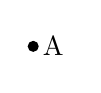
\begin{tikzpicture}[x=1cm,y=0.4cm]
    \fill (0,0) circle[radius=2pt];
    \draw (0,0) coordinate (a) node[right] {A};
\end{tikzpicture}
& Point 点& Point A 点A\\ \hline
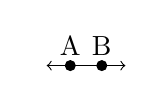
\begin{tikzpicture}[x=1cm,y=0.4cm]
	\draw (-0.5,0) coordinate (a0) node[left] {};
    \draw (-0.2,0) coordinate (a) node[above] {A};
    \draw (0.2,0) coordinate (b) node[above] {B};
    \draw (0.5,0) coordinate (b0) node {};
    \fill (-0.2,0) circle[radius=2pt];
     \fill (0.2,0) circle[radius=2pt];
     \draw[->](a) -- (a0);
    \path[draw] (a) -- (b);
    \draw[->] (b) -- (b0);
\end{tikzpicture}
& Line 直线& Line AB 直线AB\\ \hline
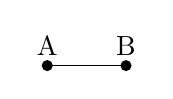
\begin{tikzpicture}[x=1cm,y=0.4cm]
    \draw (-0.5,0) coordinate (a) node[above] {A};
    \draw (0.5,0) coordinate (b) node[above] {B};
    \fill (-0.5,0) circle[radius=2pt];
     \fill (0.5,0) circle[radius=2pt];
    \path[draw] (a) -- (b);
\end{tikzpicture}
& Segment 线段& Segment AB 线段AB\\ \hline
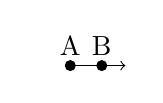
\begin{tikzpicture}[x=1cm,y=0.4cm]
	\draw (-0.5,0) coordinate (a0) node[left] {};
    \draw (-0.2,0) coordinate (a) node[above] {A};
    \draw (0.2,0) coordinate (b) node[above] {B};
    \draw (0.5,0) coordinate (b0) node {};
    \fill (-0.2,0) circle[radius=2pt];
     \fill (0.2,0) circle[radius=2pt];
    \path[draw] (a) -- (b);
    \draw[->] (b) -- (b0);
\end{tikzpicture}
& Ray 射线& Ray AB 射线AB\\ \hline
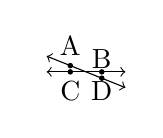
\begin{tikzpicture}[x=1cm,y=0.4cm]
	\draw (-0.5,0) coordinate (a0) node[left] {};
    \draw (-0.2,0) coordinate (a) node[below] {C};
    \draw (0.2,0) coordinate (b) node[below] {D};
    \draw (0.5,0) coordinate (b0) node {};
    \fill (-0.2,0) circle[radius=1pt];
     \fill (0.2,0) circle[radius=1pt];
     \draw[->](a) -- (a0);
    \path[draw] (a) -- (b);
    \draw[->] (b) -- (b0);
    \draw (-0.5,0.5) coordinate (aa0) node[left] {};
    \draw (-0.2,0.2) coordinate (aa) node[above] {A};
    \draw (0.2,-0.2) coordinate (bb) node[above] {B};
    \draw (0.5,-0.5) coordinate (bb0) node {};
    \fill (-0.2,0.2) circle[radius=1pt];
     \fill (0.2,-0.2) circle[radius=1pt];
     \draw[->](aa) -- (aa0);
    \path[draw] (aa) -- (bb);
    \draw[->] (bb) -- (bb0);
\end{tikzpicture}
& Intersecting lines 两线相交& Two lines meet in a point 两线有一个交点\\ \hline
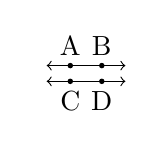
\begin{tikzpicture}[x=1cm,y=0.4cm]
	\draw (-0.5,0) coordinate (a0) node[left] {};
    \draw (-0.2,0) coordinate (a) node[below] {C};
    \draw (0.2,0) coordinate (b) node[below] {D};
    \draw (0.5,0) coordinate (b0) node {};
    \fill (-0.2,0) circle[radius=1pt];
     \fill (0.2,0) circle[radius=1pt];
     \draw[->](a) -- (a0);
    \path[draw] (a) -- (b);
    \draw[->] (b) -- (b0);
    \draw (-0.5,0.5) coordinate (aa0) node[left] {};
    \draw (-0.2,0.5) coordinate (aa) node[above] {A};
    \draw (0.2,0.5) coordinate (bb) node[above] {B};
    \draw (0.5,0.5) coordinate (bb0) node {};
    \fill (-0.2,0.5) circle[radius=1pt];
     \fill (0.2,0.5) circle[radius=1pt];
     \draw[->](aa) -- (aa0);
    \path[draw] (aa) -- (bb);
    \draw[->] (bb) -- (bb0);
\end{tikzpicture}
& Parallel lines 平行线& Line AB and CD never meet.  直线AB和CD不相交\\ \hline
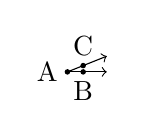
\begin{tikzpicture}[x=1cm,y=0.4cm]
    \draw (0,0) coordinate (a) node[left] {A};
    \draw (0.2,0) coordinate (b) node[below] {B};
    \draw (0.5,0) coordinate (b0) node {};
    \draw (0.2,0.2) coordinate (c) node[above] {C};
    \draw (0.5,0.5) coordinate (c0) node {};
    \fill (0,0) circle[radius=1pt];
     \fill (0.2,0) circle[radius=1pt];
      \fill (0.2,0.2) circle[radius=1pt];
    \path[draw] (a) -- (b);
    \draw[->] (b) -- (b0);
    \path[draw] (a) -- (c);
    \draw[->] (c) -- (c0);
\end{tikzpicture}
& Angle 角& Vertex: A, Sides: AB, AC 顶点:A,边:AB,AC\\ \hline
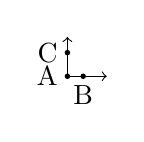
\begin{tikzpicture}[x=1cm,y=1cm]
    \draw (0,0) coordinate (a) node[left] {A};
    \draw (0.2,0) coordinate (b) node[below] {B};
    \draw (0.5,0) coordinate (b0) node {};
    \draw (0,0.3) coordinate (c) node[left] {C};
    \draw (0,0.5) coordinate (c0) node {};
    \fill (0,0) circle[radius=1pt];
     \fill (0.2,0) circle[radius=1pt];
      \fill (0,0.3) circle[radius=1pt];
    \path[draw] (a) -- (b);
    \draw[->] (b) -- (b0);
    \path[draw] (a) -- (c);
    \draw[->] (c) -- (c0);
\end{tikzpicture}
& Right Angle 直角& Right angle looks like a square. 直角两边互相垂直\\ \hline
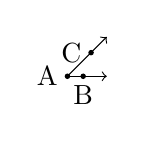
\begin{tikzpicture}[x=1cm,y=1cm]
    \draw (0,0) coordinate (a) node[left] {A};
    \draw (0.2,0) coordinate (b) node[below] {B};
    \draw (0.5,0) coordinate (b0) node {};
    \draw (0.3,0.3) coordinate (c) node[left] {C};
    \draw (0.5,0.5) coordinate (c0) node {};
    \fill (0,0) circle[radius=1pt];
     \fill (0.2,0) circle[radius=1pt];
      \fill (0.3,0.3) circle[radius=1pt];
    \path[draw] (a) -- (b);
    \draw[->] (b) -- (b0);
    \path[draw] (a) -- (c);
    \draw[->] (c) -- (c0);
\end{tikzpicture}
& Acute Angle 锐角& Acute angle is smaller than right angle. 锐角小于直角\\ \hline
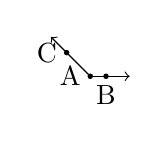
\begin{tikzpicture}[x=1cm,y=1cm]
    \draw (0,0) coordinate (a) node[left] {A};
    \draw (0.2,0) coordinate (b) node[below] {B};
    \draw (0.5,0) coordinate (b0) node {};
    \draw (-0.3,0.3) coordinate (c) node[left] {C};
    \draw (-0.5,0.5) coordinate (c0) node {};
    \fill (0,0) circle[radius=1pt];
     \fill (0.2,0) circle[radius=1pt];
      \fill (-0.3,0.3) circle[radius=1pt];
    \path[draw] (a) -- (b);
    \draw[->] (b) -- (b0);
    \path[draw] (a) -- (c);
    \draw[->] (c) -- (c0);
\end{tikzpicture}
& Obtuse Angle 钝角& Obtuse angle is larger than right angle. 钝角大于直角\\ \hline
\end{tabular}
\end{table}

\newpage

\subsection{Counting 数数}
\begin{paracol}{2}
Counting is one of the basic skills when we learn numbers. And it is the basis of arithmetic. "Skip Counting" is counting by a number that is not 1. Learning to "Skip Count" helps you count many things quickly and learn your multiplication tables. 
 
\switchcolumn[1]
数数是我们在学习了数字以后所学习的,它是所有计算的基础。除了连续的数数,我们也应该学会跳着数数。它可以帮助我们数的更快,也是学习乘法口诀的基础。
\switchcolumn[0]*
For counting problems, you should be careful that miss anything and should not count something more than once. 
\switchcolumn[1]
对于数数的问题,最重要的就是不要漏掉,不应重复,如果漏掉了要加上,如果重复了要剪掉。
\end{paracol}

\begin{example}
How many line segments in the graph? 数一数下图中有多少条线段?
\begin{center}
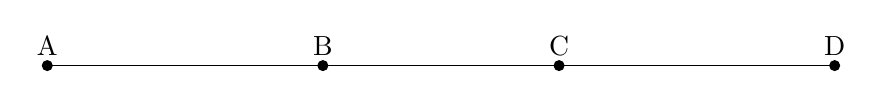
\begin{tikzpicture}[x=5cm,y=0.4cm]
    \draw (-1,0) coordinate (a) node[above] {A};
    \draw (-0.3,0) coordinate (b) node[above] {B};
    \draw (0.3,0) coordinate (c) node[above] {C};
    \draw (1,0) coordinate (d) node[above] {D};
     \fill (-1,0) circle[radius=2pt];
    \fill (-0.3,0) circle[radius=2pt];
     \fill (0.3,0) circle[radius=2pt];
     \fill (1,0) circle[radius=2pt];
    \path[draw] (a) -- (b) -- (c) -- (d);
\end{tikzpicture}
\end{center}
\end{example}
\begin{solution}
\begin{itemize}
\item Continuous points 连续两点:AB, BC, CD
\item Every other points 隔一个点:AC, BD
\item Every other two points 隔两点:AD
\end{itemize}
Therefore, there are 6 line segments. 因此,总共有6条线段。
\end{solution}

\begin{example}
Several people are in one row. There are 6 people in front of David and 8 people behind. How many people are there in this row? 一些人排成一列,在David的前面有6人,后面有8人,问这列队共有多少人?
\end{example}
\begin{solution}
As shown in the graph, 如图所示:
\begin{center}
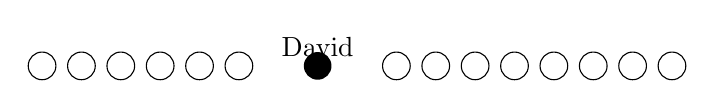
\begin{tikzpicture}[x=5cm,y=0.4cm]
    \draw (0,0) coordinate (a) node[above] {David};
     \draw (-0.7,0) circle[radius=5pt];
     \draw (-0.6,0) circle[radius=5pt];
     \draw (-0.5,0) circle[radius=5pt];
     \draw (-0.4,0) circle[radius=5pt];
     \draw (-0.3,0) circle[radius=5pt];
     \draw (-0.2,0) circle[radius=5pt];
    \fill (0,0) circle[radius=5pt];
    \draw (0.2,0) circle[radius=5pt];
    \draw (0.3,0) circle[radius=5pt];
    \draw (0.4,0) circle[radius=5pt];
    \draw (0.5,0) circle[radius=5pt];
    \draw (0.6,0) circle[radius=5pt];
    \draw (0.7,0) circle[radius=5pt];
    \draw (0.8,0) circle[radius=5pt];
    \draw (0.9,0) circle[radius=5pt];
\end{tikzpicture}
\end{center}

There are 15 people in the line. 总人数是15人。
\end{solution}
\newpage
\subsection{Comparing and ordering 比较与排序}
\begin{paracol}{2}
There are three relationship between two numbers: equal, greater, or less. Sorting is ordering the numbers in a line by comparing the values, or arranging something with certain requirements.
\switchcolumn[1]
两个数之间有三种关系:相等,大于和小于。排序就是把互相不等的一些数通过比较按大小顺序排列
起来,或是按照一定的要求把一些东西排列起来。
\end{paracol}
\begin{newthem}[The Greater Than, Less Than, and Equal Symbols]
The special symbols are used to show if a number is greater \bm{ $>$}, less \bm{$<$}, or $\bm{=}$.\\
$\bm{>}$,$\bm{<}$和 $\bm{=}$ 用来表示大于、小于和等于关系。
\begin{align}
\text{large number} > \text{small number} && \text{大数}>\text{小数}\\
\text{small number} < \text{large number} & &\text{小数}<\text{大数}
\end{align}
\end{newthem}

\begin{paracol}{2}
Very often we need to compare numbers to see which is the greatest or the least. The basic rules for comparing the numbers are as follows
\switchcolumn[1]
我们经常需要比较两个数的大小。比较两个数大小的方法如下
\end{paracol}

\begin{newalg}[Rules For Comparing Two Numbers 比较两个数大小的方法]
\begin{enumerate}
\item The greater the number of digits, the greater is the number.
\item If two numbers have the same number of digits, the number with the bigger digit on the left hand side is greater.
\item If the leftmost digits are the same we compare the next digit to the right and keep doing this until the digits are different.
\end{enumerate}

\begin{enumerate}
\item 两个数位数多的数大
\item 如果两个数的数字个数相同,最左边的数字大的数大
\item 如果最左边的数字相同,就比较它右边的数字,如果还相同继续比较右边的数字,直到数字不同,数字大的数大。如果数字都相同则两个数一样大。
\end{enumerate}
\end{newalg}

\begin{example}
Compare these numbers 比较下面的数字
$$
\begin{matrix}
a) 675,\ \  67\quad & b)  2,148,\ \ 3,147  & c)  2,178,345,\ \ 2,178,987 & d) 492,789,100, \ \ 492,789,100
\end{matrix}
$$
\end{example}
\begin{solution}

{
\centering
\begin{tabular}{|c|p{10cm}|}
\toprule	
& \parbox[c]{10cm}{\centering Why? 原因}\\
\midrule
$675 > 67$ & The first number is 3-digit number, while second is 2-digit. 第一个数有三位,第二个数有两位\\ \hline
${\color{red}2},148 < {\color{red}3},147$ & The first digit is smaller in the first number. 第一个数首位数小\\ \hline
$2,178,{\color{red}3}45 < 2,178,{\color{red}9}87$& The first digit is the same, but the fifth digit is smller in the first number. 首位相同,但第一个数从左起第五个位数字小\\ \hline
$492,789,100=492,789,100$ & All digits are the same. 所有的位置数字相同\\
\bottomrule
\end{tabular}
}

\end{solution}

\begin{example}
List the numbers in order from least to greatest. 把下列数字从小到大排序。
$$
1\quad 5\quad 35\quad 27\quad 14\quad 36\quad 63\quad 69\quad 78\quad 87\quad 99\quad 100 
$$
\end{example}
\begin{solution}
Based on the following rules: 根据以下的原则进行排序:
\begin{enumerate}
\item 1-digit numbers $<$ 2-digit numbers $<$ 3-digit numbers. 一位数小于两位数小于三位数。
\item For 2-digit numbers, compare tens first. 两位数比较,先比较十位;十位数字相同的比较个位。
\end{enumerate}
The result is as follows 排列结果如下:
$$
1<5<14<27<35<36<63<69<78<87<99<100.
$$
\end{solution}

\begin{example}
The following are some animals and their ages. List them from young to old. 下面是一些动物的年龄,请将他们按年龄从小到大排列。

\begin{tabular}{ll}
Elephant: 80, 大象:80岁;& Giraffe: 25 长颈鹿:25岁\\
Horse: 40, 马:40岁; & Monkey: 30, 猴子:30岁\\
Tiger: 20, 老虎:20岁; & Carp: 100, 鲤鱼:100岁\\
Turtle: 170, 乌龟:170岁; & Parrot: 104, 鹦鹉:104岁
\end{tabular}
\end{example}

\begin{solution}
List the numbers from least to greast: 把数字从小到大排序,我们得到:
$$
20<25<30<40<80<100<104<170.
$$ 
Therefore, the animals are listed as 所以动物按照以下顺序排序
$$
\text{tiger} < \text{Giraffe} < \text{Monkey} < \text{Horse} < \text{Elephant} < \text{Carp} < \text{Parrot} < \text{Turtle}.
$$
$$
\text{老虎} < \text{长颈鹿} < \text{猴子} < \text{马} < \text{大象} < \text{鲤鱼} < \text{鹦鹉} < \text{乌龟}.
$$
\end{solution}

\begin{note}
From here, it is not required in the normal class. 以下为补充内容,非课本要求。
\end{note}

\begin{newprop}[transitivity 传递性]
There are three numbers. If the first number is less than the second and the second is less than the third, then the first number is less than the third number.
Similarly, if the first number is greater than the second and the second is greater than the third, then the first number is greater than the third number.

如果有三个数。如果第一个数小于第二个,第二个数小于第三个数,则第一个数小于第三个数。同样的如果第一个数大于第二个,第二个数大于第三个数,则第一个数大于第三个数。
\end{newprop}

\begin{example}
Put $1,2,3,4$ into the circles in the following graph to satisfy all of the relationships between each two circles. 把 $1, 2, 3, 4$ 填入下图中的小圆圈里是的图中所示的不等关系成立。
\begin{center}
\begin{tikzpicture}[thick]
  \node[draw,circle,minimum size = 0.8cm] at (0,0)(a){};
  \node[draw,circle,minimum size = 0.8cm] at (50,50)(b) {};
  \node[draw,circle,minimum size = 0.8cm] at (50,-50) (c) {};
  \node[draw,circle,minimum size = 0.8cm] at (100,0)(d) {};
  
  \node[inner sep=0,minimum size=0] at (40,0)(k0) {$>$}; % invisible node
  \node[inner sep=0,minimum size = 0,rotate=45] at (25,25)(k1) {$>$};
  \node[inner sep=0,minimum size = 0,rotate=-45] at (25,-25)(k2) {$>$};
  \node[inner sep=0,minimum size = 0,rotate=90] at (50,-15)(k3) {$>$};
  \node[inner sep=0,minimum size = 0,rotate=-45] at (75,25)(k4) {$<$};
  \node[inner sep=0,minimum size = 0,rotate=45] at (75,-25)(k5) {$>$};
  % draw arrows
  \draw[] (a) to (k1);
  \draw[] (k1) to (b);
  \draw[] (a) to (k2);
  \draw[] (k2) to (c);
  \draw[] (a) to (k0);
  \draw[] (k0) to (d);
  \draw[] (b) to (k3);
  \draw[] (k3) to (c);
  \draw[] (b) to (k4);
  \draw[] (k4) to (d);
  \draw[] (c) to (k5);
  \draw[] (k5) to (d);
\end{tikzpicture}
\end{center}
\end{example}
\begin{solution}
\begin{paracol}{2}
\begin{itemize}
\item Since the number in the left circle is greater than the other three, it is $4$.
\item Since the number in the upper circle is less than the other three, it should be $1$.
\item The number in the lower circle is greater than the number in the right circle. Therefore, the lower one is $3$ and the right one is $2$.
\end{itemize}
\switchcolumn[1]
\begin{itemize}
\item 最左端的小圆圈中应填的数都大于其他三个小圆圈中应填的数,所以应填最大的数$4$;
\item 最上面的小圆圈应填的数最小,所以应填$1$;
\item 最下面的小圆圈应填的数大于右边的小圆圈应填的数,所以最下面圆圈应填$3$,最右边应填$2$。
\end{itemize}
\end{paracol}
\begin{center}
\begin{tikzpicture}[thick]
  \node[draw,circle,minimum size = 0.8cm] at (0,0)(a){4};
  \node[draw,circle,minimum size = 0.8cm] at (50,50)(b) {1};
  \node[draw,circle,minimum size = 0.8cm] at (50,-50) (c) {3};
  \node[draw,circle,minimum size = 0.8cm] at (100,0)(d) {2};
  
  \node[inner sep=0,minimum size=0] at (40,0)(k0) {$>$}; % invisible node
  \node[inner sep=0,minimum size = 0,rotate=45] at (25,25)(k1) {$>$};
  \node[inner sep=0,minimum size = 0,rotate=-45] at (25,-25)(k2) {$>$};
  \node[inner sep=0,minimum size = 0,rotate=90] at (50,-15)(k3) {$>$};
  \node[inner sep=0,minimum size = 0,rotate=-45] at (75,25)(k4) {$<$};
  \node[inner sep=0,minimum size = 0,rotate=45] at (75,-25)(k5) {$>$};
  % draw arrows
  \draw[] (a) to (k1);
  \draw[] (k1) to (b);
  \draw[] (a) to (k2);
  \draw[] (k2) to (c);
  \draw[] (a) to (k0);
  \draw[] (k0) to (d);
  \draw[] (b) to (k3);
  \draw[] (k3) to (c);
  \draw[] (b) to (k4);
  \draw[] (k4) to (d);
  \draw[] (c) to (k5);
  \draw[] (k5) to (d);
\end{tikzpicture}
\end{center}
\end{solution}

\begin{example}
\begin{paracol}{2}
There are 6 friends working on one projects. Here are some information about their ages.
\begin{enumerate}
\item Peter and Andrew are the same age.
\item James is older than John, but younger than Peter.
\item Philip is younger than Peter and James, but older than John.
\item Andrew is younger than Thomas.
\end{enumerate}
Please list them by age and find out who is the oldest and who is the youngest.
\switchcolumn[1]
六个小伙伴一起在做一个任务。下面是关于他们年龄的一些线索:
\begin{enumerate}
\item 彼得和安德烈同岁;
\item 雅各比约翰年龄大,但比彼得小;
\item 腓力比彼得和雅各小,但比约翰大;
\item 安德烈比多马年纪小。
\end{enumerate}
请按照年龄给他们排序。并回答谁年龄最大?谁年龄最小?
\end{paracol}
\end{example}
\begin{solution}
\begin{paracol}{2}
Based on the information, we have
\begin{enumerate}
\item Based on 1, Peter $=$ Andrew.
\item Based on 2, Peter $>$James $>$ John. \\
Therefore, Peter  $=$ Andrew $>$James $>$ John
\item Based on 3, Peter $>$ James $>$ Philip $>$ John. Therefore, 
Peter $=$ Andrew  $>$ James $>$ Philip $>$ John.
\item Based on 4, Thomas $>$Andrew.
\end{enumerate}
We have listed them by ages as follows
\switchcolumn[1]
根据他们年龄的线索,我们可以判断:
\begin{enumerate}
\item 由1,彼得$=$安德烈;
\item 由2,彼得$>$雅各$>$约翰。\\所以,彼得$=$安德烈$>$雅各$>$约翰;
\item 由3,彼得$>$雅各$>$腓力$>$约翰。所以,彼得$=$安德烈$>$雅各$>$腓力$>$约翰;
\item 由4,多马$>$安德烈。
\end{enumerate}
我们按照年龄给他们排序如下:
\end{paracol}
\begin{center}
Thomas $>$ Peter $=$ Andrew  $>$ James $>$ Philip $>$ John\\
多马$>$彼得$=$安德烈$>$雅各$>$腓力$>$约翰
\end{center}
\begin{paracol}{2}
Therefore, Thomas is the oldest and John is the youngest.
\switchcolumn[1]
所以多马年龄最大,约翰年龄最小。
\end{paracol}
\end{solution}

\begin{exercise}
\begin{paracol}{2}
\begin{enumerate}
\item 1
\item 2
\item 3
\item 4
\end{enumerate}
\switchcolumn[1]
\begin{enumerate}
\item 1
\item 2
\item 3
\item 4
\end{enumerate}
\end{paracol}
\end{exercise}
   \newpage
\subsection{Rounding 四舍五入}
\begin{paracol}{2}
Rounding means making a number simpler but keeping its value close to what it was. The result is less accurate, but easier to use. 
\switchcolumn[1]
近似是寻找一个和原来的数接近的看起来比较“简单”的数。它不精确,但是相对简单。
\switchcolumn[0]*
There are several different methods for rounding. Here we look at the common method, the one used by most people.
\switchcolumn[1]
有许多种不同的近似方法,通常我们用的方法是四舍五入。其方法如下:
\end{paracol}

\begin{newalg}[How to Round Numbers 四舍五入方法]
\begin{enumerate}
\item Decide which is the last digit to keep
\item Leave it the same if the next digit is less than 5 (this is called rounding down)
\item But increase it by 1 if the next digit is 5 or more (this is called rounding up)
\end{enumerate}

\begin{enumerate}
\item 决定要保持的位
\item  如果其下一位小于5,保持这位的数字(向下近似)
\item  如果其下一位大于等于5,则这位数字加1(向上近似)
\end{enumerate}
\end{newalg}

\begin{example}
Round 73 to the nearest 10 把73近似到十位
\end{example}
\begin{solution}
\begin{paracol}{2}
Since $7$ is the tens position, we want to keep it. The next digit is $3$, which is less than $5$. Therefore, no change is needed. The answer is $70$.
\switchcolumn[1]
因为十位上是 $7$,这是我们要保持的数。而其个位为$3$,小于$5$。所以十位不用加一就是 $7$。所以,四舍五入到十位是 $70$。
\end{paracol}
\end{solution}

\begin{example}
Round 191 to the nearest 100 把$191$近似到百位
\end{example}
\begin{solution}
\begin{paracol}{2}
Since $1$ is the hundreds position, we want to keep it. The next digit is $9$, which is greater than $5$. Therefore, increase $1$ to $2$. The answer is $200$.
\switchcolumn[1]
因为百位上是 $1$,这是我们要保持的数。而其十位为$9$,大于$5$。所以百位加一就是 $2$。所以,四舍五入到百位是 $200$。
\end{paracol}
\end{solution}
\newpage

\section{Addtion and subtraction 数的加减法}
\subsection{Basic facts of addition and subtraction 加减法基础}
\begin{paracol}{2}
These basic strategies can help you remember addition facts for small numbers.
\begin{enumerate}
\item Count on from the greater number. For example, $6+3$. Count on from $6$ 3 times: $7,8,9$. So $6+3=9$.
\item Use doubles. For example, $8+7$. Since $7+7=14$, $8+7 = 14+1=15$.
\item Use 10 to add 8 or 9. For example, $9+5 = 10+4 = 14$.
\end{enumerate}
\switchcolumn[1]
对于小数的加法,有如下的技巧可以帮助我们:
\begin{enumerate}
\item 从大数开始数数、例如: $6+3$。从$6$开始数三次:$7,8,9$.所以$6+3=9$.
\item 翻倍。例如:$8+7$。因为$7+7=14$,$8+7=7+7+1=15$。
\item 利用10做8或9相关的加法。例如:$9+5=10+4=14$。
\end{enumerate}
\switchcolumn[0]*
These basic strategies can help you remember subtraction facts for small numbers.
\begin{enumerate}
\item Count back from the greater number. For example, $6-2$. Count back from $6$ twice: $5,4$. So $6-2=4$.
\item Count up from the lesser number. For example, $7-5$. Count on from $5$ to $7$: $6,7$. So $7-5=2$.
\item Use 10 to subtract 8 or 9. For example, $16-9 = 16-10+1 = 7$.
\end{enumerate}
\switchcolumn[1]
对于小数的减法,有如下的技巧可以帮助我们:
\begin{enumerate}
\item 从大数倒数。例如, $6-2$. 从 $6$ 倒数两个数: $5,4$. 所以 $6-2=4$。
\item 从小数数。例如,$7-5$. 从 5 数到 7: $6,7$. 所以 $7-5=2$。
\item 利用10计算减 8 或 9. 例如, $16-9 = 16-10+1 = 7$。
\end{enumerate}
\switchcolumn[0]*
For the addition and subtraction of large numbers, the column method can be useful. The way to do the column method is as follows:
\begin{description}
\item [Step 1: ] Create columns for each place value. From right to left, we will create a ones column,  tens column, hundreds column, and so on. And we align the numbers by the place value. For example, ones of the first number will align with ones of the second. 
\item [Step 2: ]  Add/subtract the digits in each column starting from ones. 
\item [Step 3: ] Borrowing/ Carrying numbers. If the sum of the digits is 2-digit number, we have to carry a number to the next column. If the top digit in any of the columns is smaller than the bottom digit then we have to borrow from the next column.
\end{description}
\switchcolumn[1]
对于较大的数的加减法,我们会利用竖式来帮助我们计算。其方法如下:
\begin{description}
\item [第1步: ] 列竖式。数的每一位对其。例如第一个数的个位和第二个数的个位要对其。
\item [第2步:] 从个位起,诸位数字相加。
\item [Step 3: ] 处理进位/借位。加法中如果某位数字加和大于$10$,则要向下一位进位。减法中如果某位数字被减数较小,则需要向上一位借位。
\end{description}
\end{paracol}
\begin{example}
238+126
\end{example}
\begin{solution}
$$
\begin{array}{lccc}
&hundreds&tens&ones\\
&\text{百位}& \text{十位}&\text{个位}\\
&2&3&8\\
+&1&2&6\\
\hline
&&&
\end{array}
\Rightarrow
\begin{array}{lccc}
&hundreds&tens&ones\\
&\text{百位}& \text{十位}&\text{个位}\\
&2&3&{\color{red} \bm8}\\
+&1&\ \  2_{{\color{red} \bm 1}}&{\color{red} \bm6}\\
\hline
&&&{\color{red} \bm 4}
\end{array}
$$
$$
\Rightarrow
\begin{array}{lccc}
&hundreds&tens&ones\\
&\text{百位}& \text{十位}&\text{个位}\\
&2&{\color{red} \bm 3}&8\\
+&1&\ \  {\color{red} \bm 2_{1}}&6\\
\hline
&&{\color{red} \bm 6}&4
\end{array}
\Rightarrow
\begin{array}{lccc}
&hundreds&tens&ones\\
&\text{百位}& \text{十位}&\text{个位}\\
&{\color{red} \bm2}& 3&8\\
+& {\color{red} \bm 1}&\ \ 2_{1}&6\\
\hline
&{\color{red} \bm 3}& 6&4
\end{array}
$$
$238+126 = 364.$
\end{solution}
\begin{example}
126-109
\end{example}
\begin{solution}
$$
\begin{array}{lccc}
&hundreds&tens&ones\\
&\text{百位}& \text{十位}&\text{个位}\\
&&&\\
&1&2&6\\
-&1&0&9\\
\hline
&&&
\end{array}
\Rightarrow
\begin{array}{lccc}
&hundreds&tens&ones\\
&\text{百位}& \text{十位}&\text{个位}\\
 & & {\color{red}\bm 1}&{\color{red} 16}\\
&1&\bcancel{{\color{red}\bm2}}&\bcancel{\color{red}\bm 6}\\
-&1&0&9\\
\hline
&&&{\color{red}\bm 7}
\end{array}
$$
$$
\Rightarrow
\begin{array}{lccc}
&hundreds&tens&ones\\
&\text{百位}& \text{十位}&\text{个位}\\
 & & {\color{red}\bm 1}&16\\
&1&\bcancel{{\color{red}\bm2}}&\bcancel{6}\\
-&1&{\color{red}\bm 0}&9\\
\hline
&&{\color{red}\bm 1}&7
\end{array}
\Rightarrow
\begin{array}{lccc}
&hundreds&tens&ones\\
&\text{百位}& \text{十位}&\text{个位}\\
 & & 1&16\\
&{\color{red}\bm 1}&\bcancel{2}&\bcancel{6}\\
-&{\color{red}\bm 1}&0&9\\
\hline
&\bcancel{\color{red}\bm 0}&1&7
\end{array}
$$
$126-109 = 17.$
\end{solution}
   \newpage
\subsection{Three or more addends 多个数字加法}
\begin{paracol}{2}
When there are thre or more addends, adding them one by one is the basic method. However there are also some tricks we can use to help solve
the problem more quickly. All of the tricks are based on Theorem \ref{thm:commutative}. We can add the easy addends first. 
\switchcolumn[1]
当计算三个或以上数的加法时,逐项相加是最基本的方法。但是对于一些有特殊特点的计算,有一些计算技巧可以来帮助我们。所有的技巧都是根据定理\ref{thm:commutative}。我们可以先计算简单的加和。
\end{paracol}
\begin{newthem}[Commutative property of addtion 加法交换律]
\label{thm:commutative}
changing the order of the addends does not change the result.\\
改变加法各项的顺序,计算结果不变。
\end{newthem}

\paragraph{Looking for a sum of 10  凑十法}
\ \  

\begin{paracol}{2}
We already know that the addition of the following $5$ pairs is $10$. We can use these results to do the computation quickly. 
\switchcolumn[1]
我们已经知道,下面的五组成对的数相加之和都等于$10$。利用这些结果可以使计算又快又准。
\end{paracol}
$$
\begin{aligned}
1+9=9+1=10,\quad & 2+8=8+2=10,\quad & 3+7=7+3=10\\
4+6=6+4=10,\quad & 5+5=10.
\end{aligned}
$$
\begin{example}
1+2+3+4+5+6+7+8+9+10
\end{example}
\begin{solution}
\begin{paracol}{2}
As the basic method, we can add them one by one.
\switchcolumn[1]
对于这道题,基础的方法是从左往右逐项相加。
\end{paracol}
$$
\begin{aligned}
1+2=3,\quad & 3+3=6,\quad & 6+4=10,\\
10+5=15,\quad & 15+6=21,\quad, & 21+7 = 28,\\
28+8=36,\quad & 36+9=45,\quad,& 45+10 = 55.
\end{aligned}
$$
\begin{paracol}{2}
The advantage of this method is that we can get all of the intermedia results. However it is complecated and easy to make mistakes. If one addition in one of the steps is wrong, it will be wrong after. And it is really difficult to find out where it goes wrong. The new method which looking for the sum of 10 could fix this problem.
\switchcolumn[1]
这种逐项相加的方法,好处是可以得到每一步的结果,但缺点是麻烦,容易出错;而且一步出错,以后步步都错。并且很难检查错误。若是利用凑十法,就可以克服这种缺点。
\end{paracol}

\begin{center}
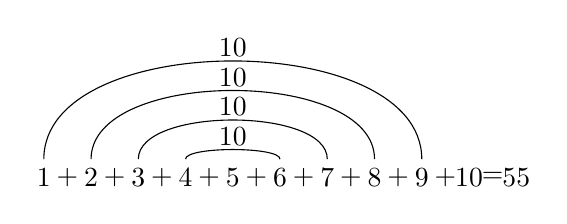
\begin{tikzpicture}[auto, node distance=0.3cm]
\node[] (1) {1};
\node[] (p1) [ right of=1] {$+$};
\node[] (2) [ right of=p1] {2};
\node[] (p2) [ right of=2] {$+$};
\node[] (3) [ right of=p2] {3};
\node[] (p3) [ right of=3] {$+$};
\node[] (4) [ right of=p3] {4};
\node[] (p4) [ right of=4] {$+$};
\node[] (5) [ right of=p4] {5};
\node[] (p5) [ right of=5] {$+$};
\node[] (6) [ right of=p5] {6};
\node[] (p6) [ right of=6] {$+$};
\node[] (7) [ right of=p6] {7};
\node[] (p7) [ right of=7] {$+$};
\node[] (8) [ right of=p7] {8};
\node[] (p8) [ right of=8] {$+$};
\node[] (9) [ right of=p8] {9};
\node[] (p9) [ right of=9] {$+$};
\node[] (10) [ right of=p9] {10};
\node[] (e) [ right of=10] {$=$};
\node[] (sum) [ right of=e] {55};
\draw (1)  .. controls +(up:1.9cm) and +(up:1.9cm) .. node [above=-2pt]{10} (9);
\draw (2)  .. controls +(up:1.4cm) and +(up:1.4cm) .. node[above=-2pt]{10} (8);
\draw (3)  .. controls +(up:0.9cm) and +(up:0.9cm) .. node[above=-2pt]{10} (7);
\draw (4)  .. controls +(up:0.4cm) and +(up:0.4cm) .. node[above=-2pt]{10} (6);
\end{tikzpicture}
\end{center}
\end{solution}

\paragraph{Looking for a sum of a whole number  凑整法}
\ \  

\begin{paracol}{2}
Some number pairs could add up to tens or hundreds. For example
\switchcolumn[1]
有些数相加之和是整十、整百的数,如:
\end{paracol}

\begin{align*}
1+19&=20, \quad & 11+19&=30,\\
12+28&=40, \quad & 12+38&=50,\\
23+37&=60, \quad & 33+37&=70,\\
34+46&=80, \quad & 44+46&=90,\\
15+85&=100, \quad & 45+55&=100.
\end{align*}

\begin{paracol}{2}
These results could help us in the computation.
\switchcolumn[1]
巧用这些结果,可以使那些较大的数相加又快又准。
\end{paracol}

\begin{example}
$1+3+5+7+9+11+13+15+17+19$
\end{example}
\begin{solution}
\begin{center}
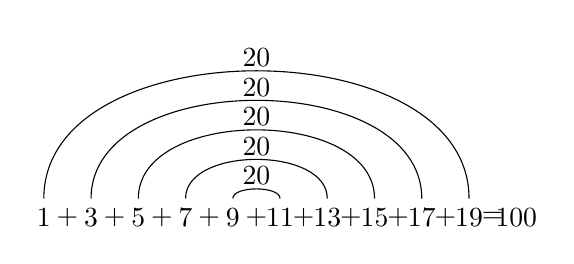
\begin{tikzpicture}[auto, node distance=0.3cm]
\node[] (1) {1};
\node[] (p1) [ right of=1] {$+$};
\node[] (3) [ right of=p1] {3};
\node[] (p2) [ right of=3] {$+$};
\node[] (5) [ right of=p2] {5};
\node[] (p3) [ right of=5] {$+$};
\node[] (7) [ right of=p3] {7};
\node[] (p4) [ right of=7] {$+$};
\node[] (9) [ right of=p4] {9};
\node[] (p5) [ right of=9] {$+$};
\node[] (11) [ right of=p5] {11};
\node[] (p6) [ right of=11] {$+$};
\node[] (13) [ right of=p6] {13};
\node[] (p7) [ right of=13] {$+$};
\node[] (15) [ right of=p7] {15};
\node[] (p8) [ right of=15] {$+$};
\node[] (17) [ right of=p8] {17};
\node[] (p9) [ right of=17] {$+$};
\node[] (19) [ right of=p9] {19};
\node[] (e) [ right of=19] {$=$};
\node[] (sum) [ right of=e] {100};
\draw (1)  .. controls +(up:2.4cm) and +(up:2.4cm) .. node [above=-2pt]{20} (19);
\draw (3)  .. controls +(up:1.9cm) and +(up:1.9cm) .. node[above=-2pt]{20} (17);
\draw (5)  .. controls +(up:1.4cm) and +(up:1.4cm) .. node[above=-2pt]{20} (15);
\draw (7)  .. controls +(up:0.9cm) and +(up:0.9cm) .. node[above=-2pt]{20} (13);
\draw (9)  .. controls +(up:0.4cm) and +(up:0.4cm) .. node[above=-2pt]{20} (11);
\end{tikzpicture}
\end{center}
\end{solution}

\begin{example}
$2+13+25+44+18+37+56+75$
\end{example}
\begin{solution}
\begin{center}

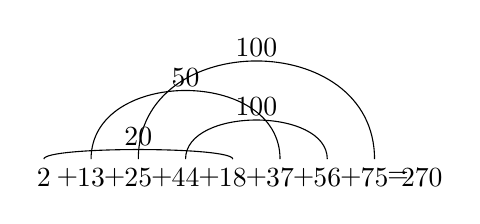
\begin{tikzpicture}[auto, node distance=0.3cm]
\node[] (2) {2};
\node[] (p1) [ right of=2] {$+$};
\node[] (13) [ right of=p1] {13};
\node[] (p2) [ right of=13] {$+$};
\node[] (25) [ right of=p2] {25};
\node[] (p3) [ right of=25] {$+$};
\node[] (44) [ right of=p3] {44};
\node[] (p4) [ right of=44] {$+$};
\node[] (18) [ right of=p4] {18};
\node[] (p5) [ right of=18] {$+$};
\node[] (37) [ right of=p5] {37};
\node[] (p6) [ right of=37] {$+$};
\node[] (56) [ right of=p6] {56};
\node[] (p7) [ right of=56] {$+$};
\node[] (75) [ right of=p7] {75};
\node[] (e) [ right of=75] {$=$};
\node[] (sum) [ right of=e] {270};
\draw (25)  .. controls +(up:1.9cm) and +(up:1.9cm) .. node [above=-2pt]{100} (75);
\draw (13)  .. controls +(up:1.4cm) and +(up:1.4cm) .. node[above=-2pt]{50} (37);
\draw (44)  .. controls +(up:0.9cm) and +(up:0.9cm) .. node[above=-2pt]{100} (56);
\draw (2)  .. controls +(up:0.4cm) and +(up:0.4cm) .. node[above=-2pt]{20} (18);
\end{tikzpicture}
\end{center}

\end{solution}
   \newpage
\subsection{Mixed calculation 加减混合运算}

\paragraph{Changing the order of operations  改变运算顺序}
\ \  

\begin{paracol}{2}
Sometimes, it is convinient to change the order of operations in the mixed equation with only addition and subtraction.
\switchcolumn[1]
在只有加减运算的算式中,有时改变加、减的运算顺序可使计算显得十分巧妙!
\end{paracol}

\begin{example}
$10-9+8-7+6-5+4-3+2-1$
\end{example}
\begin{solution}
\begin{paracol}{2}
If this question is added or subtracted in order from left to right, it is possible to draw a correct result. However,  it is more complicated  and easier to make a mistake. If you change the order of the operations, doing the subtraction first, the computation will be easier. The formula in parentheses indicates  calculating first.
\switchcolumn[1]
这题如果从左到右按顺序进行加减运算,是能够得出
正确结果的。但因为算式较长,多次加减又繁又慢且容易
出错。如果改变一下运算顺序,先减后加,就使运算显得
非常“漂亮”。下式括号中的算式表示先算。
\end{paracol}
$$
\begin{aligned}
&10-9+8-7+6-5+4-3+2-1\\
=&(10-9)+(8-7)+(6-5)+(4-3)+(2-1)\\
=&1+1+1+1+1 = 5.\\
\end{aligned}
$$

\end{solution}

\paragraph{Changing the order of terms with the sign  带着“+”、“-”号搬家}
\ \  

\begin{example}
$1-2+3-4+5-6+7-8+9-10+11$
\end{example}
\begin{solution}
\begin{paracol}{2}
How to compute $1-2$? To make it simple. We can move $+3$ to the front of $-2$. And similarly we can move $+5$ to the front of $-4$. We can simplify the computation with this technique. When you move the terms, just remember move with the sign.
\switchcolumn[1]
这题只有加减运算,而且1-2不够减。我们可以采用
带着加减号搬家的方法解决。要注意每个数自己的符号就
是这个数前面的那个“+”号或“-”号,搬家时要带着符
号一起搬。,把“+3”搬到“-2”的前面,把
“+5” 搬到了“-4” 的前面, …… 把“+11” 搬到了
“-10”的前面,这就叫带着符号搬家。巧妙利用这种搬
法,可以使计算简便。
\end{paracol}
$$
\begin{aligned}
&1-2+3-4+5-6+7-8+9-10+11\\
=&1+3-2+5-4+7-6+9-8+11-10\\
=&1+(3-2)+(5-4)+(7-6)+(9-8)+(11-10)\\
=&1+1+1+1+1+1=6
\end{aligned}
$$
\end{solution}
   \newpage

\section{Multiplication and division 数的乘除法}
\subsection{Basic facts of multiplication 乘法的基础}
\begin{paracol}{2}
Multiplication could be thought as a repeated addition. The multiplication of two numbers is equivalent to adding as many copies of one of them, the multiplicand, as the value of the other one, the multiplier. Consider the following
\switchcolumn[1]
乘法是可以用加法来表示的。两个数相乘相当于把被乘数加乘数次。例如
\end{paracol}
$$
8\times 4 = 32 \Leftrightarrow 8+8+8+8 = 32.
$$
\begin{paracol}{2}
Multiplicand and multiplier are called factors of the result. 
\switchcolumn[1]
乘数和被乘数都是乘积的因子。
\switchcolumn[0]*
For the mutiplication within 10, it is better to remember all of the results. 
\switchcolumn[1]
我们最好能都熟练的掌握10以内的数的乘法的结果。
\end{paracol}

\begin{figure}[!hbtp]
\centering
\includegraphics[width=0.7\textwidth]{timesanddivisiontablechart.jpg}
\caption{Multiplication chart\label{figur:multichart}}
\end{figure}


\begin{figure}[!hbtp]
\centering
\includegraphics[width=0.6\textwidth]{99multi.jpg}
\caption{九九乘法口诀表\label{figur:multichart1}}
\end{figure}

\subsection{Long multiplication  乘法竖式}

\begin{paracol}{2}
Long multiplication is a method used to solve the multiplication problems with large numbers. One thing can really help you in long multiplication is if you know the multiplication chart by heart. This will speed up your work and make it more accurate. 
\switchcolumn[1]
乘法竖式是用来计算较大数的乘法。如果我们可以牢记上面的乘法表,可以帮助我们更快速准确的进行竖式运算。
\end{paracol}

\paragraph{Multi-digit number times 1-digit number 多位数乘一位数}
\ \ 

\begin{paracol}{2}
The key of the multiplication is that multiplying each place value of the multi-digit number by the one-digit number and suming up the results.
\switchcolumn[1]
如果是多位数乘一位数,就用多位数中的每一位分别乘那个一位数,然后把结果相加。
\switchcolumn[0]*
\begin{description}
\item [{\bf Step 1:} ] write down the numbers on top of each other. Make sure  align the numbers on the right.
\item [{\bf Step 2:} ] Multiply each place value of the multiplicand by the 1-digit multiplier. 
\item [{\bf Step 3:} ] Align the result with the corresponding place. For exampe, multiply ones by the 1-digit number, then align the result with ones. Add the carry on numbers from the previous.
\end{description}
\switchcolumn[1]
\begin{description}
\item [{\bf 第一步:} ] 写竖式,相同数位对齐;
\item [{\bf 第二步:} ] 多位数每一位上的数分别与这个一位数相乘,从多位数个位起;
\item [{\bf 第三步:} ] 乘到哪一位就把结果写在哪一位数相应的位置上。注意加上上次计算的进位。
\end{description}
\end{paracol}

\begin{example}
$284\times 3$
\end{example}
%\multicolumn{3}{c}{\fcolorbox{black}{black}{\color{white}\ \ \ Step 1\ \ \ }}\\
\begin{solution}
$$
\begin{array}{lccc}
&2&8&4\\
\times&&&3\\
\hline
&&&
\end{array}
\Rightarrow
\begin{array}{lccc}
&2&8&{\color{red} \bm 4}\\
\times&&_{\color{red}1}&{\color{red} \bm 3}\\
\hline
&&&{\color{red} \bm 2}
\end{array}
$$
$$
\Rightarrow
\begin{array}{lccc}
&2&{\color{red} \bm 8}&4\\
\times&_{\color{red} \bm 2}&_{1}&{\color{red} \bm 3}\\
\hline
&&{\color{red} \bm 5}&2\\
\end{array}
\Rightarrow
\begin{array}{lccc}
&{\color{red} \bm2}& 8&4\\
\times&_{2}&_{1}&{\color{red} \bm 3}\\
\hline
&{\color{red} \bm 8}& 6&4
\end{array}
$$
$284\times 3= 864.$
\end{solution}

\paragraph{Multi-digit number times multi-digit number 多位数乘多位数}
\ \  

\begin{paracol}{2}
The multiplication bewteen two multi-digit numbers is based on the multiplication between multi-digit number and 1-digit number. The rule is as follows.
\switchcolumn[1]
多位数多位数乘法法则是基于多位数一位数的乘法。其法则如下:
\switchcolumn[0]*
\begin{description}
\item [{\bf Step 1:} ] write down the numbers on top of each other. It is better to write down the number with more digits on the top.
\item [{\bf Step 2:} ] Multiply the multiplicand by ones of the multiplier and align the ones of the results to the ones under the line. Then multiply the multiplicand by tens of the multiplier and align the ones of the results to the tens under the line. And so on.
\item [{\bf Step 3:} ] Sum all of the results up.
\end{description}
\switchcolumn[1]
\begin{description}
\item [{\bf 第一步:} ] 写竖式,最好把数位较多的乘数写在上面作为被乘数,数位较少的写在下面;
\item [{\bf 第二步:} ] 用被乘数与乘数的个位相乘,把相乘得到的积的末位写在个位上;然后再与十位上的数相乘写在十位上,... ...
\item [{\bf 第三步:} ] 把每次乘得的数相加得到最终结果。
\end{description}
\end{paracol}

\begin{example}
$125\times 124$
\end{example}
\begin{solution}
$$
\begin{array}{lccc}
&1&2&5\\
\times&1&2&4\\
\hline
&&&
\end{array}
\Rightarrow
\begin{array}{lccc}
&{\color{red} \bm 1}&{\color{red} \bm 2}&{\color{red} \bm 5}\\
\times&1&2&{\color{red} \bm 4}\\
\hline
&{\color{red} \bm 5}&{\color{red} \bm 0}&{\color{red} \bm 0}
\end{array}
$$
$$
\Rightarrow
\begin{array}{ccccc}
&&{\color{red} \bm 1}&{\color{red} \bm 2}&{\color{red} \bm 5}\\
\times&&1&{\color{red} \bm 2}&4\\
\hline
&&5&0&0\\
&{\color{red} \bm 2}&{\color{red} \bm 5}&{\color{red} \bm 0}&\\
&&&&\\
&&&&
\end{array}
\Rightarrow
\begin{array}{ccccc}
&&{\color{red} \bm 1}&{\color{red} \bm 2}&{\color{red} \bm 5}\\
\times&&{\color{red} \bm 1}&2&4\\
\hline
&&5&0&0\\
&2&5&0&\\
{\color{red} \bm 1}&{\color{red} \bm 2}&{\color{red} \bm 5}&&\\
&&&&
\end{array}
\Rightarrow
\begin{array}{ccccc}
&&1&2&5\\
\times&&1&2&4\\
\hline
&&5&0&0\\
&2&5&0&\\
1&2&5&&\\
\hline
{\color{red} \bm 1}&{\color{red} \bm 5}&{\color{red} \bm 5}&{\color{red} \bm 0}&{\color{red} \bm 0}
\end{array}
$$
$125\times 124= 15,500.$
\end{solution}

\begin{paracol}{2}
There are some tricks to help do the multiplication faster and easier.

1. If there are zeros at the end of the number, we can leave them and multiply the remaining numbers. Then add the zeros. 
\switchcolumn[1]
要提高计算速度有以下一些技巧。

1. 末尾有0的数的乘法。可以先把0前面的数相乘再添0,得出结果。
\end{paracol}

\begin{example}
$2800\times 130$
\end{example}
\begin{solution}
$$
\begin{array}{cccc:cc}
&&2&8&0&\\
\times&&1&3&0&\\
\hline
&&8&4&&\\
&2&8&&&\\
\hline
&3&6&4&0&0\\
\end{array}
$$
$2800\times 130=36400$.
\end{solution}

\begin{paracol}{2}
2. If there are repeat numbers in the multiplier, you do not need to compute it again. 
\switchcolumn[1]
2. 当乘数有重复的数字时,不必重复相乘,可以直接写出后面的结果。只是要注意对齐。
\end{paracol}
\begin{example}
$315\times 66$
\end{example}
\begin{solution}
$$
\begin{array}{ccccc}
&&3&1&5\\
\times&&&6&6\\
\hline
&1&8&9&0\\
1&8&9&0&\\
\hline
2&0&7&9&0\\
\end{array}
$$
$315\times 66=20790$.
\end{solution}
   \newpage
\subsection{Basic facts of division 除法的基础}
\begin{paracol}{2}
The division of two natural numbers is the process of calculating the number of times one number is contained within another one. Division is the inverse of multiplication. For example, since $4\times 5 = 20$, $20\div 5 = 4$. In division, the dividend is divided by the divisor to get a quotient. In the above example, 20 is the dividend, five is the divisor, and four is the quotient. In some cases, the divisor may not be contained fully by the dividend. 
\switchcolumn[1]
除法可以看成“重复的减法”,其的本质是计算一个数需要减另一个数多少次才能变成零。除法是减法的逆运算。例如:$4\times 5 = 20$,所以 $20\div 5 = 4$。除法中,是被除数除以除数,其结果为商数。在上面的例子中$20$是被除数,$5$是除数,$4$是商数。
\switchcolumn[0]*
Sometimes this remainder is added to the quotient as a fractional part, but in the context of integer division, where numbers have no fractional part, the remainder is kept separately or discarded.
\switchcolumn[1]
有时会出现被除数不能够被除数整除的情况,即有余数。余数可以继续计算成为商数的一部分,但现在(整数除法)我们会把它单独写出来或者忽略掉。
\end{paracol}

\begin{paracol}{2}
In order to do the division for large numbers, we have to know:
\begin{enumerate}
\item multiplication charts (at least fairly well)
\item basic division concept, based on multiplication tables (for example $28 \div 7$ or $56 \div 8$)
\item basic division with remainders (for example $54 \div 7$ or $23 \div 5$)
\end{enumerate}
\switchcolumn[1]
如果要学习较大数的除法,我们需要做到如下:
\begin{enumerate}
\item 熟练掌握九九乘法表
\item 利用乘法表计算除法 (例如 $28 \div 7$ or $56 \div 8$)
\item 知道如何计算基本的带余数的除法 (例如 $54 \div 7$ or $23 \div 5$)
\end{enumerate}
\end{paracol}

\subsection{Long division  除法竖式}

\begin{paracol}{2}
Long division is an algorithm that repeats the basic steps of
1) Divide; 2) Multiply; 3) Subtract; 4) Drop down the next digit. Here are the basic procedure\cite{Longdiv}:
\switchcolumn[1]
除法竖式的算法是在重复 1) 除; 2) 乘; 3) 减; 4) 拉下一位 这样的过程。其基本算法如下\cite{Longdiv}::
\end{paracol}

\begin{paracol}{2}
\begin{enumerate}
\item Divide
\begin{enumerate}
\item {\bf Set up the equation.} Write the dividend on the right, under the division symbol, and the divisor to the left on the outside. The quotient will eventually go on top, right above the dividend. Leave yourself plenty of space below the equation to carry out multiple subtraction operations.
\item {\bf Divide the first digit.} Working from left to right, determine how many times the divisor can go into the first digit of the dividend without exceeding it.
\item {\bf Divide the first two digits.} If the divisor is a larger number than the first digit, determine how many times the divisor goes into the first two digits of the dividend without exceeding it. If your divisor has more than two digits, you'll have to expand out even further.
\item {\bf Enter the first digit of the quotient.} Put the number of times the divisor goes into the first digit (or digits) of the dividend above the appropriate digit(s).
\end{enumerate}
\item Multiply
\begin{enumerate}
\item {\bf Multiply the divisor.} The divisor should be multiplied by the number you have just written above the dividend.
\item {\bf Record the product.} Put the result of your multiplication in step 1 beneath the dividend.
\item {\bf Draw a line.} A line should be placed beneath the product of your multiplication
\end{enumerate}
\item subtract
\begin{enumerate}
\item {\bf Subtract the product.} Subtract the number you just wrote below the dividend from the digits of the dividend directly above it. Write the result beneath the line you just drew.
\item {\bf Bring down the next digit.} Write the next digit of the dividend after result of your subtraction operation.
\end{enumerate}
\item {\bf Repeat the whole process.} Divide the new number by your divisor, and write the result above the dividend as the next digit of the quotient.
\end{enumerate}
\switchcolumn[1]
\begin{enumerate}
\item 除
\begin{enumerate}
\item {\bf 建立竖式。} 被除数写在除号下面,除数写在除号左边。商数将写在除号上边。所以在建立竖式时在上方留些空间。\\ \\ \\ \\ 
\item {\bf 除第一位。} 从被除数的最左一位开始。试验出最大的数使得这个数乘以除数小于第一位。\\ \\ 
\item {\bf 除前两位} 如果除数比第一位大, 就试验出最大的数使得这个数乘以除数小于前两位。注意,如果除数也是一个多位数,那么我们就需要更多位使得比除数大。\\ \\ 
\item {\bf 记下商数的第一位。} 把前面试验得到的数字写到商数,数字要与计算的被除数最后一位数字对齐。\\ 
\end{enumerate}
\item 乘
\begin{enumerate}
\item {\bf 乘除数} 用除数乘以上步记下的数字。\\ \\ 
\item {\bf 记录结果} 把结果写在被除数下面,结果要个上步使用的被除数数字对齐。
\item {\bf 划线。} 画一条线在刚才计算的结果下面。\\ 
\end{enumerate}
\item 减
\begin{enumerate}
\item {\bf 减。} 用被除数对应的位置减去刚才计算的结果。 把结果写到线的下方。\\ \\ 
\item {\bf 写下被除数后面的数字} 把被除数后面的数字写到刚才的计算结果后面。\\ 
\end{enumerate}
\item {\bf 重复前面的过程} 重新用除数除新上面写下的数字。把新试验出的数字写到商数位置的上一个数字右面。
\end{enumerate}
\end{paracol}

\paragraph{Dividing a number by a 1-digit number 一位数除法}
\ \ 

\begin{example}
$148\div 21$
\end{example}
%\multicolumn{3}{c}{\fcolorbox{black}{black}{\color{white}\ \ \ Step 1\ \ \ }}\\
\begin{solution}
$$
\arraycolsep=0pt
\begin{array}{rccc}
&&&\\
\cline{2-4}
3&{\Big)}\ 2\quad&\quad8\quad&\quad5\\
&&&
\end{array}
\Rightarrow
\begin{array}{rccc}
&&&\\
\cline{2-4}
3&{\Big)}\ {\color{red}\ 2}\quad&\quad8\quad&\quad5\\
&&&
\end{array}
\Rightarrow
\begin{array}{rccc}
&&\quad {\color{red}9}\quad&\\
\cline{2-4}
3&{\Big)}\ {\color{red}\ 2}\quad&\quad{\color{red}8}\quad&\quad5\\
&&&
\end{array}
$$
$$
\arraycolsep=0pt
\Rightarrow
\begin{array}{rccc}
&&\quad {\color{red}9}\quad&\\
\cline{2-4}
{\color{red}\ 3}&{\Big)}\ \ 2\quad&\quad8\quad&\quad5\\
&\quad{\color{red}2}\quad&\quad{\color{red}7}\quad&\\
\hline
&&&
\end{array}
\Rightarrow
\begin{array}{rccc}
&&\quad 9\quad&\\
\cline{2-4}
3&{\Big)}\ \ {\color{red}2}\quad&\quad{\color{red}8}\quad&\quad5\\
&\quad{\color{red}2}\quad&\quad{\color{red}7}\quad&\\
\hline
&&\quad{\color{red}1}\quad&
\end{array}
\Rightarrow
\begin{array}{rccc}
&&\quad 9\quad&\\
\cline{2-4}
3&{\Big)}\ \ 2\quad&\quad8\quad&\quad5\\
&\quad2\quad&\quad7\quad&\quad{\color{red} \downarrow}\\
\hline
&&\quad1\quad&\quad{\color{red} 5}
\end{array}
$$
$$
\arraycolsep=0pt
\Rightarrow
\begin{array}{rccc}
&&\quad 9\quad&\quad{\color{red} 5}\\
\cline{2-4}
{\color{red}3}&{\Big)}\ \ 2\quad&\quad8\quad&\quad5\\
&\quad2\quad&\quad7\quad&\quad\downarrow\\
\hline
&&\quad{\color{red}1}\quad&\quad{\color{red} 5}\\
&&&\\
&&&
\end{array}
\Rightarrow
\begin{array}{rccc}
&&\quad 9\quad&\quad5\\
\cline{2-4}
3&{\Big)}\ \ 2\quad&\quad8\quad&\quad5\\
&\quad2\quad&\quad7\quad&\quad\downarrow\\
\hline
&&\quad{\color{red}1}\quad&\quad{\color{red} 5}\\
&&\quad{\color{red} 1}\quad&\quad{\color{red} 5}\\ \hline
&&&\quad{\color{red} 0}
\end{array}
$$
$285\div 3= 95.$
\end{solution}

\paragraph{Dividing a number by a multi-digit number 多位数除法}
\ \  

\begin{example}
$148\div 21$
\end{example}
%\multicolumn{3}{c}{\fcolorbox{black}{black}{\color{white}\ \ \ Step 1\ \ \ }}\\
\begin{solution}
\input longdiv.tex
$$
\longdiv{148}{21}
$$
$148\div 21= 7\ R\  1.$
\end{solution}

   \newpage
\subsection{Exponentiation 指数运算}
\begin{paracol}{2}
Exponentiation is a special operation for writing a product in which all of the numbers being multiplied are the same. For example, $2\times 2\times 2\times 2$ can be written as $2^4$. We call the entire expression $2^4$ a {\bf power}, specifically the power of $2$. The number on the bottom is the base. The number on top is the exponent. 
\switchcolumn[1]
指数运算是多个相同数字的乘积的另一种表达方式。例如:$2\times 2\times 2\times 2$ 可以写成 $2^4$。$2^4$ 被称为指数运算,或2的幂。指数运算中,在下面的数字被称为底数,在上面的数字被称为指数。
\switchcolumn[0]*
When the exponent is $2$, we call it a square which means the product of a number ans itself. For example, $4^2$ is called "four squared". When the exponent is $3$, we call it a cube. So $6^3$ is called "six cubed".
\switchcolumn[1]
当指数为$2$时,我们称为平方。一个数的平方是此数与它的本身相乘所得的乘积。例如:$4^2$称为4的平方。当指数为$3$时,我们称为立方。如$6^3$称为6的立方。
\end{paracol}

\begin{example}
\begin{tabular}{cccc}
a. $10^2$& b. $3^5$ & c. $5^6$ & d. $10^7$
\end{tabular}
\end{example}
\begin{solution}
\begin{align*}
a.\quad & 10^2 = 10\times 10 = 100.\\
b.\quad & 3^5 = 3\times 3\times 3\times 3\times 3 = 243.\\
c.\quad & 5^6 = 5\times 5\times 5\times 5\times 5\times 5 = 125\times 125 = 15625.\\
d.\quad & 10^7 = 10,000,000\\
\end{align*}
\end{solution}

\begin{newprop}[Product of powers 幂相乘]
{\bf Same exponent}: The product of two powers with the same exponent is the product of the two base with the same exponent. For example, \\
同指数幂相乘,指数不变,底数相乘。例如:
$$
3^3\times 4^3 = (3\times 4)^3
$$
{\bf Same base:} The exponent of the product of two powers with the same base is the sum of the two powers. The base is the same.\\
同底数幂相乘,底数不变,指数相加
$$
4^3\times 4^5 = 4^{3+5}
$$
\end{newprop}

\begin{example}
Explain why 
$$
 3^3\times 4^3 = (3\times 4)^3, \quad 4^3\times 4^5 = 4^{3+5}
$$
\end{example}
\begin{solution}
\begin{align*}
&3^3\times 4^3 \\
=& (3\times 3\times 3) \times (4\times 4\times 4)\\
=& (3\times 4) \times (3\times 4) \times (3\times 4)\\
=& (3\times 4)^3
\end{align*}
\begin{align*}
&4^3\times 4^5\\
=& (4\times 4\times 4) \times (4\times 4\times 4\times 4\times 4)\\
=& 4\times 4\times 4 \times 4\times 4\times 4\times 4\times 4\\
=& 4^8\\
=& 4^{3+5}
\end{align*}
\end{solution}

\begin{newprop}[Quotient of powers 幂相除]
{\bf Same exponent}: The quotient of two powers with the same exponent is the quotient of the two base with the same exponent. For example, \\
同指数幂相除,指数不变,底数相除。例如:
$$
6^3\div 2^3 = (6\div 2)^3
$$
{\bf Same base:} The exponent of the quotient of two powers with the same base is the subtraction of the two powers. The base is the same.\\
同底数幂相除,底数不变,指数相减。例如:
$$
4^5\div 4^3 = 4^{5-3}
$$
\end{newprop}

\begin{example}
Explain why 
$$
6^3\div 2^3 = (6\div 2)^3, \quad 4^5\div 4^3 = 4^{5-3}
$$
\end{example}
\begin{solution}
\begin{align*}
&6^3\div 2^3  \\
=& (6\times 6\times 6) \div (2\times 2\times 2)\\
=& 6\times 6\times 6 \div 2\div 2\div 2\\
=& (6\div 2) \times (6\div 2) \times (6\div 2)\\
=& (6\div 2)^3
\end{align*}
\begin{align*}
&4^5\div 4^3 \\
=& (4\times 4\times 4\times 4\times 4)\div (4\times 4\times 4)\\
=& 4\times 4\times 4 \times 4\times 4\div 4\div 4\div 4\\
=& 4^2\\
=& 4^{5-3}
\end{align*}
\end{solution}

\begin{newprop}[Power of powers 幂的幂]
When raising a power to a power in an exponential expression, you find the new power by multiplying the two powers together. For example, \\
一个数的幂的幂等于这两个幂相乘。例如:
$$
(6^3)^3 = 6^{3\times 3}
$$
\end{newprop}

\begin{example}
Simplify. Rewrite the expression in the form $5^{*}$. 化简。把下面表达式写成 $5^{*}$的形式。
$$
(5^3)^2
$$
\end{example}
\begin{solution}
$$
(5^3)^2 = 5^{3\times 2} = 5^6.
$$

\end{solution}\begin{newprop}[Zero-Exponent Rule 零次幂]
Any number raised to the zero power is 1. For example, \\
任何数的零次幂等于1。例如:
$$
181^0 = 1.
$$
\end{newprop}
\newpage

\subsection{factoring 因数分解}
\begin{paracol}{2}
Factors are the numbers you multiply together to get another number. There can be many factors of a number.
\switchcolumn
两个正整数相乘,那么这两个数都叫做积的因数,或称为约数。一个数可以有许多的因数。
\end{paracol}

\begin{example}
Find all factors of $12$ 找到$12$的所有因数\\
\end{example}
\begin{solution}
\begin{paracol}{2}
Since 
\switchcolumn 
因为
\end{paracol}
$$
1\times 12 = 12, \quad 2\times 6 = 12,\quad 3\times 4 = 12
$$
\begin{paracol}{2}
$1, 2, 3, 4, 6$ and $12$ are factors of $12$.
\switchcolumn 
 $1, 2, 3, 4, 6, 12$ 是$12$的因数。
\end{paracol}
\end{solution}

\begin{newdef}[Prime and composite number 质数(素数)和合数]
A {\bf Prime number} is a whole number greater than 1 that cannot be made by multiplying two smaller whole numbers. A whole number greater than 1 that is not prime is called a {\bf composite number}.\\
质数(素数)为在大于1的自然数中,除了1和此整数自身外两个因数,无法被其他自然数整除的数。合数是除了1和它本身还有其它正因数。
\end{newdef}

\begin{note}
$1$ is neither prime number nor composite number. $1$既不是质数也不是合数。
\end{note}

\begin{paracol}{2}
Here is some examples of prime numbers.
\switchcolumn
下面是一些小的质数:
\end{paracol}
$$
2,\quad 3\quad 5,\quad 7,\quad 9,\quad 11,\quad 13,\quad 17,\quad 19,\quad 23,\quad 29,\quad 31,\quad 37,\quad 41,\cdots
$$



\begin{paracol}{2}
Integer factorization is the decomposition of a composite number into a product of smaller integers. If these integers are further restricted to prime numbers, the process is called prime factorization.
\switchcolumn
整数分解是将一个正整数写成几个因数的乘积。如果所有的因数是质数则称为质因数分解。
\end{paracol}

\begin{example}
What are the prime factors of $30$? 把30分解质因数。
\end{example}
\begin{solution}
\begin{paracol}{2}
It is best to start working from the smallest prime number, which is $2$, so 
\switchcolumn 
要找到所有的的质因数,最好从最小的质数开始试。
\end{paracol}
$$
30\div 2 = 15.
$$
\begin{paracol}{2}
$15$ is a composite number, but it cannot be divided by $2$. Therefore, let us try $3$.
\switchcolumn 
$15$是合数,但它不能被$2$整除,所以我们试着除以$3$。
\end{paracol}
$$
15\div 3 = 5.
$$
\begin{paracol}{2}
So we have the answer:
\switchcolumn 
所以题目的答案是:
\end{paracol}
$$
30 = 2\times 3\times 5. 
$$
\end{solution}

\begin{example}
The sum of two prime numbers is $40$. In all of the possible choices of these two numbers, what is the maximum  product? 两个质数的和是40,求这两个质数的乘积的最大值是多少?
\end{example}
\begin{solution}
\begin{paracol}{2}
All possible prime number pairs are as follows
\switchcolumn 
把40表示为两个质数的和,共有三种形式
\end{paracol}
$$
40 = 17 + 23 = 11+29 = 3+37.
$$
\begin{paracol}{2}
Since
\switchcolumn 
因为
\end{paracol}
$$
17\times 23 = 391 > 11\times 29 = 319> 3\times 37 = 111.
$$
\begin{paracol}{2}
The maximum product is $391$.
\switchcolumn 
这两个质数的最大乘积是391。
\end{paracol}
\end{solution}

\paragraph{Greatest common divisor and least common multiple 最大公约数和最小公倍数}
\ \ 

\begin{newdef}[Greatest common divisor 最大公约数]
The greatest common divisor (gcd) of two or more integers, which are not all zero, is the largest positive integer that divides each of the integers. \\
几个数公有的约数,叫做这几个数的公约数;其中最大的一个,叫做这几个数的最大公约数。
\end{newdef}

\begin{newdef}[Least common multiple 最小公倍数]
The least common multiple (lcm) of two or more integers is the smallest positive integer that is divisible by each of the integers.  \\
几个数公有的倍数,叫做这几个数的公倍数;其中最小的一个,叫做这几个数的最小公倍数。
\end{newdef}

\begin{newdef}[Coprimes 互质数]
Coprimes is a pair of numbers not having any common factors other than 1.  \\
如果两个数的最大公约数是1,那么这两个数叫做互质数。
\end{newdef}

\begin{paracol}{2}
There are several ways to find the gcd. \\ 
\begin{itemize}
\item Method of exhaustion
\item Prime factorization
\item Euclid's algorithm
\end{itemize}
\switchcolumn 
计算两个数的最大公因数有许多不同的方法:
\begin{itemize}
\item 穷举法
\item 因数分解
\item 辗转相除法
\end{itemize}
\end{paracol}


\begin{paracol}{2}
{\bf Method of exhaustion:} List all of the factors for each of the integers and choose the largest one as gcd. In practice, this method is only feasible for small numbers.
\switchcolumn 
{\bf 穷举法:}分别列出两整数的所有约数,并找出最大的公约数。这种方法只针对较小的数。
\end{paracol}

\begin{example}
用一个数去除60、75,都能整除,这个数最大是多少?
\end{example}
\begin{solution}[Method of exhaustion 穷举法]
\begin{paracol}{2}
The factors of these three numbers are
\switchcolumn 
这两个数的因子分别为:
\end{paracol}
\begin{align*}
60:\ & 1,2,3,4,5,6,10,12,{\color{red} 15},20,30,60\\
75:\ & 1, 3, 5, {\color{red} 15}, 25, 75 
\end{align*}
\begin{paracol}{2}
Therefore, the largest number is 15.
\switchcolumn 
这个数最大是15。
\end{paracol}
\end{solution}

\begin{paracol}{2}
{\bf Prime factorization:} Compute the prime factorization of each of the integers and find the "overlap" of the expressions. gcd is the product of the common factors. In practice, this method is only feasible for small numbers; computing prime factorizations in general takes far too long.
\switchcolumn 
{\bf 因数分解:}分别列出两数的素因数分解式,并计算共同项的乘积。这种方法只针对较小的数,对于大数的因式分解通常比较困难。
\end{paracol}

\begin{solution}[Prime factorization 因数分解]

\begin{paracol}{2}
The prime factorizationof these three numbers are
\switchcolumn 
这三个数的因式分解分别为:
\end{paracol}
\ \\
\begin{align*}
60=& 2\times 2\times 3\times 5\\
75:=&3\times 5\times 5
\end{align*}

\begin{paracol}{2}
The common factors are $3$ and $5$. Therefore, the largest number is $3\times 5 =15$.
\switchcolumn 
共同的因子是:3,5。这个数最大是$3\times 5 =15$。
\end{paracol}
\end{solution}

\begin{paracol}{2}
{\bf Euclid's algorithm:} Divide the large number by the small number to get the remainder. And divide the divisor by the remainder to get the new remainder. Repeat this prodecure until the remainder is zero. Then gcd is the last divisor.  Euclid's algorithm is very efficient for large numbers. The total number of steps needed is less or equal than the number of digits of the smaller number. 
\switchcolumn 
{\bf 辗转相除法:}两数相除,取余数重复进行相除,直到余数为$0$时,前一个除数即为最大公约数。辗转相除法处理大数时非常高效,它需要的步骤不会超过较小数的位数(十进制下)的五倍。
\end{paracol}

\begin{newalg}[Euclid's algorithm 辗转相除法]
\begin{enumerate}
\item Divide the large number by the small number to get the remainder;
\item Divide the divisor by the remainder to get the new remainder;
\item Repeat step 2, until the remainder is 0;
\item The gcd is the divisor of the last step.
\end{enumerate}

\begin{enumerate}
\item 大数除以小数取余数;
\item 上一步的除数除以上一步的余数取余数;
\item 重复上一步知道余数为零;
\item 前一个除数即为最大公约数。
\end{enumerate}
\end{newalg}

\begin{solution}[Euclid's algorithm 辗转相除法]
\begin{align*}
75\div 60 = & 1 \ldots 15 \\ 
60\div {\color{red} 15} = & 4
\end{align*}

\begin{paracol}{2}
 Therefore, the largest number is $15$.
\switchcolumn 
这个数最大是$15$。
\end{paracol}
\end{solution}
\newpage

\subsection{Even and odd numbers 奇数和偶数}
\begin{paracol}{2}
Even numbers can be divided evenly into groups of two. Therefore, Any whole number that can be divided exactly by 2 is an even number. Odd numbers can NOT be divided evenly into groups of two. Any whole number that cannot be divided exactly by 2 is an odd number.
\switchcolumn
整数可以分成奇数和偶数两大类.能被2整除的数叫做偶数,不能被2整除的数叫做奇数。
\end{paracol}

\begin{note}
Zero is even numbers becasue $0\div 2 = 0$. 因为0能被2整除,所以0是偶数。
\end{note}

\begin{paracol}{2}
The arithmetic of even and odd numbers are as following 
\switchcolumn
奇数与偶数的运算性质如下:
\end{paracol}

\begin{table}[!hbtp]
\begin{center}
\begin{tabular}{rrrr}
Even$+$Even$=$Even &偶数$+$偶数$=$偶数 & Even$-$Even$=$Even & 偶数$-$偶数$=$偶数 \\ 
odd$+$\,\:odd$=$Even &奇数$+$奇数$=$偶数 & odd$-$\,\:odd$=$Even & 奇数$-$奇数$=$偶数 \\ 
Even$+$\,\:odd$=$\,\:odd &偶数$+$奇数$=$奇数 & Even$-$\,\:odd$=$\,\:odd & 偶数$-$奇数$=$奇数 \\ 
odd$+$Even$=$\,\:odd &奇数$+$偶数$=$奇数 & odd$-$Even$=$\,\:odd & 奇数$-$偶数$=$奇数 \\ 
Even$\times$Even$=$Even &偶数$\times$偶数$=$偶数 & odd$\times$\,\:odd$=$\,\:odd &奇数$\times$奇数$=$奇数 \\ 
odd$\times$Even$=$Even &奇数$\times$偶数$=$偶数 & Even$\times$\,\:odd$=$Even & 偶数$\times$奇数$=$偶数 \\ 
\multicolumn{2}{l}{The sum of even numbers of odd is even} & \multicolumn{2}{l}{偶数个奇数相加得偶数}\\
\multicolumn{2}{l}{The sum of odd numbers of odd is even} & \multicolumn{2}{l}{奇数个奇数相加得奇数}\\
\end{tabular}
\end{center}
\end{table}

\begin{example}
Is $1+2+\cdots+2018$ even or odd? \\
$1+2+\cdots+2018$ 是奇数还是偶数?
\end{example}
\begin{solution}
\begin{paracol}{2}
Since $2018\div 2 = 1009$. From $1$ to $2018$, there are $1009$ even number and $1009$ odd number. The sum of $1009$ even number is even and the sum of  $1009$ odd number is odd. Therefore, $1+2+\cdots+2018$  is odd.
\switchcolumn
因为 $2018\div 2 = 1009$. 从 $1$ 到 $2018$, 有$1009$个偶数,$1009$个奇数。 $1009$个偶数的和是偶数,$1009$个奇数的和是奇数。因为奇数加偶数是奇数,所以原式的和一定是奇数。
\end{paracol}
\end{solution}
\newpage


\section{Arithmetic of integers 四则混合运算}
\subsection{Order of operations 运算顺序}
\begin{paracol}{2}
It is important to know the order of operations when you have different arithmetic in one equation. 
\switchcolumn[1]
对于四则混合运算,掌握运算顺序是十分重要的。
\end{paracol}

\begin{table}[htp]
\centering
\definecolor{LightRed}{rgb}{1,0.88,0.88}
\definecolor{LightCyan}{rgb}{0.88,1,1}
\definecolor{LightGreen}{rgb}{0.88,1,0.88}
\definecolor{LightPink}{rgb}{1,0.88,1}
\begin{tabular}{>{\columncolor{LightCyan}}c>{\columncolor{LightRed}}c>{\columncolor{LightGreen}}c>{\columncolor{LightGreen}}c>{\columncolor{LightPink}}c>{\columncolor{LightPink}}c}
{\color{blue}\bf P} & {\color{red}\bf E} & {\color{green!40!black}\bf M}& {\color{teal} \bf D} & {\color{purple} \bf A} &{\color{magenta} \bf S}\\
{\color{blue}\bf P}arenthesis & {\color{red}\bf E}xponents & {\color{green!40!black}\bf M}ultiplication & {\color{teal} \bf D}ivision & {\color{purple} \bf A}ddition & {\color{magenta} \bf S}ubtraction \\
{\color{blue}括号} & {\color{red} 指数} & {\color{green!40!black} 乘法} & {\color{teal} 除法} & {\color{purple} 加法} & {\color{magenta} 减法}\\
$\xrightarrow[\text{自左至右计算}]{\textsl{From left to right}}$ & $\xrightarrow[\text{自左至右计算}]{\textsl{From left to right}}$  & \multicolumn{2}{>{\columncolor{LightGreen}}c}{$\xrightarrow[\text{自左至右计算}]{\textsl{From left to right}}$}  & \multicolumn{2}{>{\columncolor{LightPink}}c}{$\xrightarrow[\text{自左至右计算}]{\textsl{From left to right}}$}\\
{\color{blue}$ (),[],\{\}$} & {\color{red} $ \ ^2, \sqrt{\ \ }$} & {\color{green!40!black} $\times, *, \cdot$} & {\color{teal} $\div, /$} & {\color{purple} $+$} & {\color{magenta} $-$}
\end{tabular}
\end{table}

\begin{example}
$150 - 50\times 2 +18$
\end{example}
\begin{solution}
\begin{align*}
&150 - {\color{red} 50\times 2} +18& \text{Compute multiplication first 先计算乘法}\\
=&{\color{red} 150 - 100} + 18 & \text{Compute addition and subtraction }\\
=& {\color{red} 50 + 18} & \text{from left to right 从左至右计算加减}\\
=& 68
\end{align*}
\end{solution}

\begin{example}
$800-600\div (25\times 4)$
\end{example}
\begin{solution}
\begin{align*}
&800-600\div {\color{red}(25\times 4)}&   \text{{\color{blue}\bf P}arenthesis\  {\color{blue}括号} }\\
=&800 - {\color{red}600\div 100} &  \text{{\color{green!40!black}\bf M}ultiplication\& {\color{teal} \bf D}ivision\  {\color{green!40!black} 乘法}  {\color{teal} 除法}}\\
=& {\color{red}800 - 6}& \text{{\color{purple} \bf A}ddition \& {\color{magenta} \bf S}ubtraction\ {\color{purple} 加法}{\color{magenta} 减法}}\\
=& 796
\end{align*}

\end{solution}
\newpage

\subsection{Properties 四则运算的运算律}

\begin{paracol}{2}
The summary of the properties of the arithmetics are as follows.
\switchcolumn[1]
四则运算的规律如下:
\end{paracol}

\begin{newprop}[Commutative property of addition 加法交换律]
If the order of the addends changes, the sum will stay the same.\\
加法各项交换顺序,其和不变。
$$
8+7 = 15, \quad 7+8=15.
$$
\end{newprop}

\begin{example}
Find the missing number 空格中填入缺少的数。
$$
\begin{matrix}
5+6 = \underline{\quad} + 5 & 50+4 = \underline{\quad} + 50\\
125+70 = \underline{\quad} + 125 & 17655+6 = \underline{\quad} + 17655
\end{matrix}
$$
\end{example}
\begin{solution}
$$
\begin{matrix}
5+6 = \underline{\color{red} 6} + 5 & 50+4 = \underline{\color{red} 4} + 50\\
125+70 = \underline{\color{red} 70} + 125 & 17655+6 = \underline{\color{red} 6} + 17655
\end{matrix}
$$
\end{solution}

\begin{newprop}[Associative property of addition 加法结合律]
If the grouping of the addends changes, the sum will stay the same. \\
三个数相加,先把前两个数相加,或者先把后两个数相加,和不变。
$$
(7+8)+9 = 24, \quad 7+(8+9) = 24.
$$
\end{newprop}

\begin{example}
Find the missing number 空格中填入缺少的数。
$$
\begin{matrix}
(2+3)+4= \underline{\quad} + (3+4) & (50+4)+7 = 50+(\underline{\quad}+7)\\
12+(2+5) = (12+\underline{\quad}) + 5 & 1+(6+2) = (1+6)+\underline{\quad}
\end{matrix}
$$
\end{example}
\begin{solution}
$$
\begin{matrix}
(2+3)+4= \underline{\color{red} 2} + (3+4) & (50+4)+7 = 50+(\underline{\color{red} 4}+7)\\
12+(2+5) = (12+\underline{\color{red} 2}) + 5 & 1+(6+2) = (1+6)+\underline{\color{red} 2}
\end{matrix}
$$
\end{solution}

\begin{newprop}[Commutative property of multiplication 乘法交换律]
If the order of the factors changes, the product will stay the same.\\
交换乘数和被乘数的位置,乘积不变。
$$
3\times 5 = 15, \quad 5\times 3 = 15.
$$
\end{newprop}
\newpage
\begin{example}
Find the missing number 空格中填入缺少的数。
$$
\begin{matrix}
5\times6 = \underline{\quad} \times 5 & 50\times  \underline{\quad} = 7\times\underline{\quad} \\
125\times70 = 70\times \underline{\quad} & \underline{\quad} \times 6 = \underline{\quad} \times 17
\end{matrix}
$$
\end{example}
\begin{solution}
$$
\begin{matrix}
5\times6 = \underline{\color{red} 6} \times 5 & 50\times  \underline{\color{red} 7} = 7\times\underline{\color{red} 50} \\
125\times70 = 70\times \underline{\color{red} 125} & \underline{\color{red} 17} \times 6 = \underline{\color{red} 6} \times 17
\end{matrix}
$$
\end{solution}

\begin{newprop}[Associative property of multiplication 乘法结合律]
If the grouping of the factors changes, the sum will stay the same. \\
三个数相乘,先把前两个数相乘,或者先把后两个数相乘,积不变。
$$
(3\times4)\times 5 = 60, \quad 3\times(4\times5) = 60.
$$
\end{newprop}

\begin{example}
Find the missing number 空格中填入缺少的数。
$$
\begin{matrix}
(2\times3)\times 4= \underline{\quad} \times (3\times 4) & (50\times 4)\times \underline{\quad} = 50\times(\underline{\quad}\times 7)\\
12\times(7\times 5) = (\underline{\quad}\times \underline{\quad}) \times 5 & 10\times (6\times 2) = (\underline{\quad}\times 6)\times \underline{\quad}
\end{matrix}
$$
\end{example}
\begin{solution}
$$
\begin{matrix}
(2\times3)\times 4= \underline{\color{red}  2} \times (3\times 4) & (50\times 4)\times \underline{\color{red}  7} = 50\times(\underline{\color{red} 4}\times 7)\\
12\times(7\times 5) = (\underline{\color{red}  12}\times \underline{\color{red} 7}) \times 5 & 10\times (6\times 2) = (\underline{\color{red} 10}\times 6)\times \underline{\color{red}  2}
\end{matrix}
$$
\end{solution}

\begin{newprop}[Distributive law 乘法分配律]
Multiplying a number by a group of numbers added together is the same as doing each multiplication separately.\\
两个数的和与一个数相乘,可以先把它们分别与这个数相乘,再将积相加。
$$
3\times(4+5) = 3\times 4 + 3\times 5 = 27.
$$
\end{newprop}

\begin{example}
$8\times (10+2)$
\end{example}
\begin{solution}
\begin{align*}
&8\times (10+2)\\
=&8\times 10 + 8\times 2\\
=& 80 + 16\\
=& 96
\end{align*}
\end{solution}

\begin{newprop}[Identity property 恒等性质]
When we add 0 to any number, the number does not change.\\
任何一个数加零,等于这个数本身。
$$
5+0 = 5.
$$
When we multiply any number by 1, the number does not change.\\
任何数乘以零,等于这个数本身。
$$
5\times 1 = 5.
$$
\end{newprop}

\begin{paracol}{2}
We are going to simplify the calculation by using these properties. But sometimes, it might be confusing. We need to do more practice to fully understand the concept. 
\switchcolumn[1]
灵活运用各种运算律是为了帮助我们更快的计算。然而,这也很容易产生一些混淆和疑惑。建议理解和熟练要交互运用,通过练习来掌握这些计算技巧。
\switchcolumn[0]*
It is important to notice that there is no commutative and associative properties for subtraction and division. When applying the associative property, we need to transfer subtraction and division to addition and multiplication.
\switchcolumn[1]
另外,需要注意减法和除法没有交换律和结合律。如果我们需要使用结合律,我们要记住变号(减号变加号,除号变乘号)
\end{paracol}

\begin{example}
$1600\div 10\div 4\div 2$
\end{example}
\begin{solution}
It is ok to solve it step by step. 我们可以从左到右依次计算。
\begin{align*}
&1600\div 10\div 4\div 2\\
=&160\div 4\div 2\\
=&40\div 2\\
=& 20
\end{align*}
We can also combine the divisor. 我们也可以把除数一起整合后一起除。
\begin{align*}
&1600\div 10\div 4\div 2\\
=&1600\div (10\times 4\times 2)\\
=&1600\div 80\\
=& 20
\end{align*}
\end{solution}
   \newpage

\section{Number patterns 数字的规律}
\subsection{Number patterns 数字的规律}
\begin{paracol}{2}
Patterns are all around us! Finding and understanding patterns gives us great power. With patterns we can learn to predict the future, discover new things and better understand the world around us. Number pattern is a list of numbers that follow a certain sequence or pattern.
\switchcolumn
生活中处处有规律存在。能够找到并理解其中的规律能够帮助我们处理很多事情。利用这些规律可以帮助我们进行预测分析,也能够帮助我们更好的理解这个世界。数字的规律就是给出一系列有一定的规律的数字。
\end{paracol}


\begin{example}
Look at the following number sequence and fill in the missing gaps 观察下面的数列,找出规律并填下缺少的数字。
$$
1)\quad 1, 2, 3, 4, 5, \underline{\quad}, \underline{\quad} \quad\quad\quad \quad\quad\quad 2)\quad 2, 4, 6, \underline{\quad}, 10, \underline{\quad}, \underline{\quad}
$$
$$
3)\quad 2, 4, 8, \underline{\quad}, 32, \underline{\quad}, 128 \quad\quad\quad\quad\  4)\quad 1, 2, \underline{\quad}, 7, 11,  \underline{\quad}, 22
$$
$$
5)\quad 1600,\underline{\quad} , 400, 200, \underline{\quad}, 50, \underline{\quad}\quad\ 6)\quad 0, 15, \underline{\quad}, 0, 15, 30 \ \  
$$
\end{example}
\begin{solution}
\begin{paracol}{2}
1) Pattern: Addition of one.
\switchcolumn
规律:下一个是前一个数字加一。
\end{paracol}
$$
1, 2, 3, 4, 5, \underline{{\color{red}\ 6\ }}, \underline{{\color{red}\ 7\ }}
$$
\begin{paracol}{2}
2) Pattern: Addition of two.
\switchcolumn
规律:下一个是前一个数字加二。
\end{paracol}
$$
2, 4, 6, \underline{{\color{red}\ 8\ }}, 10, \underline{{\color{red}\ 12\ }}, \underline{{\color{red}\ 14\ }}
$$
\begin{paracol}{2}
3) Pattern: Doubling each time.
\switchcolumn
规律:下一个是前一个数字的两倍。
\end{paracol}
$$
2, 4, 8, \underline{{\color{red}\ 16\ }}, 32, \underline{{\color{red}\ 64\ }}, 128
$$
\begin{paracol}{2}
4) Pattern: Adding one more each time.(Fibonacci Numbers)
\switchcolumn
规律:相邻两个数字的差逐次加一。(斐波那切数列)
\end{paracol}
$$
1, 2, \underline{{\color{red}\ 4\ }}, 7, 11,  \underline{{\color{red}\ 16\ }}, 22
$$
\begin{paracol}{2}
5) Pattern: Halving each time. 
\switchcolumn
规律:下一个是前一个数字的一半。
\end{paracol}
$$
1600,\underline{{\color{red}\ 800\ }} , 400, 200, \underline{{\color{red}\ 100\ }}, 50, \underline{{\color{red}\ 25\ }}
$$
\begin{paracol}{2}
6) Pattern: Repeated pattern.
\switchcolumn
规律:三个数一组重复出现。
\end{paracol}
$$
0, 15, \underline{{\color{red}\ 30\ }}, 0, 15, 30
$$
\end{solution}

\subsection{Common number sequences 常见的一些数列}
\begin{paracol}{2}
An {\bf Arithmetic Sequence} is a sequence that the difference between one term and the next is a constant. The difference between the terms is called common difference.
\switchcolumn
等差数列:如果一个数列从第二项起,每一项与它的前一项的差等于同一个常数,这个数列就叫做等差数列,而这个常数叫做等差数列的公差。
\end{paracol}
\begin{newprop}[通项公式]
We can write an Arithmetic Sequence as a rule:
$$
\text{k-th term} = \text{first term} + \text{Common difference}\times(k-1)
$$
$$
\text{第几项} = \text{首项} + \text{公差}\times(\text{项数}-1)
$$
\end{newprop}

\begin{newprop}[项数公式]
The number of terms of the Arithmetic Sequence as can be computed by 
$$
\text{Number of terms} = (\text{last term} - \text{first term}) \div \text{Common difference} + 1
$$
$$
\text{项数} = (\text{末项} - \text{首项}) \div \text{公差} + 1
$$
\end{newprop}

\begin{newprop}[Summing an Arithmetic Series 求和公式]
To sum up the terms of this arithmetic sequence, use this formula
$$
\text{sum} = (\text{fisrt term} + \text{last term}) \times \text{Number of terms} \div 2
$$
$$
\text{总和} = (\text{首项} + \text{末项}) \times \text{项数} \div 2
$$
\end{newprop}

\begin{paracol}{2}
An {\bf Geometric Sequence} each term is found by multiplying the previous term by a constant. The difference between the terms is called common ratio.
\switchcolumn
等比数列:从第二项起,每一项与前一项的比都是一个常数,这个数列就叫做等比数列,而这个常数叫做等差数列的公比。
\end{paracol}

\begin{paracol}{2}
The {\bf  Fibonacci Sequence} is found by adding the two numbers before it together. 
\switchcolumn
斐波那契数列:数列从第三项开始,每一项都等于前两项之和。
\end{paracol}
\newpage


\chapter{Decimals and fractions 小数和分数}
\section{Decimals and fractions 小数与分数}
\subsection{Decimals 小数}
\begin{paracol}{2}
Decimals is a representation of a non-negative real numbers. The dots in the number is called decimal separator. A decimal separator is a symbol used to separate the integer part from the fractional part of a number written in decimal form.
\switchcolumn
小数,是实数的一种特殊的表现形式。小数中的圆点叫做小数点,它是一个小数的整数部分和小数部分的分界号。其中整数部分是零的小数叫做纯小数,整数部分不是零的小数叫做带小数。
\end{paracol}

\begin{figure}[!hbtp]
\begin{center}
\includegraphics[width=0.6\textwidth]{tenth.png}
      \caption{Visual representation of decimals and fractions 小数和分数的图像表示}
      \label{fig:decimalsquare}
\end{center}
\end{figure}

\begin{table}[htp]
\centering
\begin{tabular}{|p{.8cm}<{\centering}|p{.8cm}<{\centering}|p{.8cm}<{\centering}|p{.8cm}<{\centering}!{\vrule width 1.6pt}p{.8cm}<{\centering}|p{.8cm}<{\centering}|p{.8cm}<{\centering}|}
\hline
\parbox[t]{2mm}{\rotatebox[origin=c]{90}{thousands} }&
\parbox[t]{2mm}{\rotatebox[origin=c]{90}{hundred}}&\parbox[t]{2mm}{ \rotatebox[origin=c]{90}{ten}}& \parbox[t]{2mm}{\rotatebox[origin=c]{90}{ones} }&
\rotatebox[origin=c]{90}{\parbox[c]{2cm}{\centering \begin{spacing}{0.8}tenths\end{spacing}}}&\rotatebox[origin=c]{90}{\parbox[c]{2cm}{\centering \begin{spacing}{0.8}hundredths\end{spacing}}}& \rotatebox[origin=c]{90}{\parbox[c]{2cm}{\centering thousandths}}\\
\midrule
7&5&5&0&2&6&2\\
\bottomrule
\end{tabular}
\caption{7550.262: Seven thousand five hundred fifty and two hundred sixty-two thousandths\\
七千五百五十五又千分之二百六十二\label{tab:decimals}}
\end{table}

\begin{paracol}{2}
\begin{description}
\item [{\bf Finite decimals: }] A regular number, also called a finite decimal, is a positive number that has a finite decimal expansion,like $3.1465$,$0.364$,$8.3218798456$, and so on. 
\item [{\bf Repeating decimals: }] A repeating decimal, \\
 also called a recurring decimal, is a number whose decimal representation eventually becomes periodic (i.e., the same sequence of digits repeats indefinitely), like $0.\overline{142857}=0.142857142857\ldots$ and $1.8\overline{3}=1.833\ldots$. The minimum number of digits that repeats in such a number is known as the decimal period. 
\item [{\bf Nonperiodic and nonrepeating decimals: }] \ \\ Nonperiodic and nonrepeating decimal is an irrational number. An irrational number is a number that cannot be expressed as a fraction. For example, the ratio of a circle's circumference to its diameter is $\pi =3.141592653589793\ldots$.  Euler's number is $e=2.71828\ldots$.
\end{description}
\switchcolumn
\begin{description}
\item [{\bf 有限小数:}] 小数部分后有有限个数位的小数。如$3.1465$,$0.364$,$8.3218798456$等。\\ 
%有限小数都属于有理数,可以化成分数形式。
%一个最简分数可以被化作十进制的有限小数当且仅当其分母只含有质因数2或5或两者。 类似的,一个最简分数可以被化作某正整数底数的有限小数当且仅当其分母之质因数为此基底质因数的子集。
\item [{\bf 循环小数:}] 从小数部分的某一位起,一个数字或几个数字,依次不断地重复出现的小数叫做循环小数。如 $0.\overline{142857}=0.142857142857\ldots$,$1.8\overline{3}=1.833\ldots$等。这一节数字称为循环节。\\ \\ \\ \\  %循环小数亦属于有理数,可以化成分数形式。
\item [{\bf 无限不循环小数:}] 小数部分有无限多个数字,且没有依次不断地重复出现的一个数字或几个数字的小数叫做无限不循环小数,如圆周率 $\pi =3.14159265358979323\ldots$,自然对数的底数 $e=2.71828182845904\ldots$。%无限不循环小数也就是无理数,不能化成分数形式。
\end{description}
\end{paracol}

\subsection{Fractions 分数}

\begin{paracol}{2}
A fraction represents a part of a whole or, more generally, any number of equal parts. A fraction (examples:  $\frac{1}{2}$ and $17/3$) consists of an numerator displayed above a line (or before a slash), and a non-zero denominator. The numerator represents a number of equal parts, and the denominator indicates how many of those parts make up a unit or a whole. 
\switchcolumn
分数可视为将某件事物平均分成的几份中占据其中的几份。分数可以用分式来表示,例如 $\frac{1}{2}$ 和 $17/3$。其中,中间的线称为分数线。分数线上的称为分子,分数线下的数称为分母。
\end{paracol}

\begin{paracol}{2}
\begin{description}
\item [{\bf Irreducible fraction:}] An irreducible fraction is a fraction in which the numerator and denominator are integers that have no other common divisors than 1.
\item [{\bf Proper Fraction: }] The fraction is called proper if the numerator is less than the denominator. In general, a common fraction is said to be a proper fraction if the absolute value of the fraction is strictly less than one.
\item [{\bf Top-heavy/Improper Fraction: }] It is said to be an improper fraction, or sometimes top-heavy fraction,[12] if the absolute value of the fraction is greater than or equal to 1.
\item [{\bf mixed numeral: }] A mixed numeral is a traditional denotation of the sum of a non-zero integer and a proper fraction. Any such mixed fractions can be converted to an improper fraction. For example, $1\frac{1}{2}=\frac{1\times2+1}{2}=\frac{3}{2}$.
\item [{\bf unit fraction: }] A unit fraction is a number written as a fraction where the numerator is one and the denominator is a positive integer.
\end{description}
\switchcolumn
\begin{description}
\item [{\bf 最简分数(既约分数):}] 分子是整数,分母是正整数,且分子和分母互素的分数。\\ 
\item [{\bf 真分数:}] 除商小于1、大于0的分数,即分子小于分母的分数。\\ \\ \\ \\ 
\item [{\bf 假分数:}] 假分数是指除商不小于1的分数,即分子等于或大于分母的分数。\\ \\ \\ 
\item [{\bf 带分数:}] 一个整数加一个真分数,带分数可以写成假分数。例如 $1\frac{1}{2}$,就是一又二分之一,与$\frac{1\times2+1}{2}=\frac{3}{2}$等价。\\ \\ \\ 
\item [{\bf 单位分数:}] 分子为1,分母是整数的分数。
\end{description}
\end{paracol}

\paragraph{Equivalent fractions 约分、扩分及通分}
\ \ \\

\begin{paracol}{2}
Multiplying the numerator and denominator of a fraction by the same (non-zero) number results in a fraction that is equivalent to the original fraction. This is true because multiplying the numerator and denominator of a fraction by the same number is equivalent to multiplying by one, and any number multiplied by one has the same value as the original number. Dividing the numerator and denominator of a fraction by the same non-zero number will also yield an equivalent fraction. This is called reducing or simplifying the fraction. A common fraction can be reduced to lowest terms by dividing both the numerator and denominator by their greatest common divisor.
\switchcolumn
\ \\ 一个分数约分后或扩分后,其分数与原来之分数的值相等,称为等值分数。“扩分”是将一个分数的分子和分母同乘以比1大的数。 扩分后的分数和原来分数的值相等。“约分”是将一个分数的分子和分母同除以一个比1大的整数(它们的公约数)。 约分后的分数和原来分数的值相等。“通分”是利用约分或扩分,将两个分母不同的分数,分别化为同分母的分数。
\end{paracol}

\subsection{Converting between decimals and fractions 小数与分数的转化}

\begin{paracol}{2}
To change a common fraction to a decimal, do a long division of the decimal representations of the numerator by the denominator (this is idiomatically also phrased as "divide the denominator into the numerator"), and round the answer to the desired accuracy. To change a decimal to a fraction, we need to consider by the different types of decimals.
\switchcolumn[1]
把分数化为小数只需要做一个除法。用分子除以分母,然后取到小数点后相应的位数。根据小数类型的不同,有不同的方法把小数化为分数:
\switchcolumn[0]*
\begin{description}
\item [{\bf Convert finite decimals: }] To change a decimal to a fraction, write in the denominator a  $1$ followed by as many zeroes as there are digits to the right of the decimal point, and write in the numerator all the digits of the original decimal, just omitting the decimal point. For example, $12.3456 = \frac{123456}{10000}$.
\item [{\bf Converting repeating decimals to fractions}] For repeating patterns where the repeating pattern begins immediately after the decimal point, a simple division of the pattern by the same number of nines as numbers it has will suffice. For example, $0.\overline{9}=\frac{9}{9}=1$, $0.\overline{25}=\frac{25}{99}$, $0.\overline{3}=\frac{3}{9}=\frac{1}{3}$. In case leading zeros precede the pattern, the nines are suffixed by the same number of trailing zeros. In case a non-repeating set of decimals precede the pattern, we can write it as the sum of the non-repeating and repeating parts, respectively:
$0.1\overline{3}=0.1+0.0\overline{3}=\frac{3}{30}+\frac{1}{10}\frac{1}{3} = \frac{4}{30} = \frac {2}{15}$.
\item [{\bf Nonperiodic and nonrepeating decimals}] \ \\ Nonperiodic and nonrepeating decimal is an irrational number. Therefore, it cannot be converted to a fraction. 
\end{description} 
\switchcolumn
\begin{description}
\item [{\bf 有限小数化分数:}] 把有限小数去掉小数点后作为分子;分母是以“1”开头,有限小数的小数点后有几位,就在1后跟几个零。例如:$12.3456 = \frac{123456}{10000}$。\\ \\ \\ \\ 
\item [{\bf 循环小数化分数:}] 如果是纯循环小数则把循环节作为分子,循环节如果有一位,分母为9;循环节有两位,分母为99;循环节有三位,分母为999,依次类推。如 $0.\overline{9}=\frac{9}{9}=1$,$0.\overline{25}=\frac{25}{99}$, $0.\overline{3}=\frac{3}{9}=\frac{1}{3}$。混循环小数化分数则需要化为有限小数和纯循环小数之和后化简,如 $0.1\overline{3}=0.1+0.0\overline{3}=\frac{3}{30}+\frac{1}{10}\frac{1}{3} = \frac{4}{30} = \frac {2}{15}$。\\ \\ \\ \\ \\ \\ 
\item [{\bf 无限不循环小数}] 无限不循环小数为无理数,不可以化为分数。
\end{description}
\end{paracol}

\newpage

\subsection{Comparing and ordering 小数和分数的比较}
\begin{paracol}{2}
The method to compare decimals is as follows.
\switchcolumn[1]
比较两个小数的方法如下:
\end{paracol}

\begin{newalg}[Comparison of decimals 小数的比较方法]
\begin{enumerate}
\item {\bf Compare the whole numbers to the left of the decimal point.} If they are not the same, the smaller decimal number is the one with the smaller whole number.
\item {\bf Compare the whole number to the right of the decimal point.} Starting from the digit on the right of the decimal point, compare the digits. The smaller digit number is the one with the smaller whole number.
\end{enumerate}

\begin{enumerate}
\item {\bf 比较整数部分。如果整数部分不同,则整数部分小的数小。} 
\item  {\bf 比较小数部分。如果整数部分相同,再比较小数部分。小数部分第一位大的那个数就大;如果第一位上的数相同,就比较第二位上的数……依次比下去。} 
\end{enumerate}
\end{newalg}


\begin{paracol}{2}
Comparing fractions with the same denominator yields the same result as comparing the numerators. One way to compare fractions with different numerators and denominators is to find a common denominator. If two positive fractions have the same numerator, then the fraction with the smaller denominator is the larger number.
\switchcolumn[1]
如果分数的分子相同,则只需要比较两个分数的分子,分子大的分数比较大。所以分数通常的比较方法是先通分,使得两个分数的分母相同,然后比较分子。另外,如果分数的分子相同,则分母大的分数比较小。
\end{paracol}

\begin{example}
Compare these numbers 比较下面的数字
$$
\begin{matrix}
a) 2.9, \ \  3.11\quad & b)  6.51,\ \ 6.38  & c)  2.7\ \ 2.70 & d) \dfrac{6}{11}, \ \ \dfrac{8}{11} & e) \dfrac{6}{5}, \ \ \dfrac{8}{7} 
\end{matrix}
$$
\end{example}
\begin{solution}

{
\centering
\begin{tabular}{|c|p{10cm}|}
\toprule	
& \parbox[c]{10cm}{\centering Why? 原因}\\
\midrule
${\color{red}2}.9 < {\color{red}3}.11$ & The numbers to the left of the decimal point of the first number is smaller. 第一个数的整数部分小\\ \hline
$6.{\color{red}5}1 > 6.{\color{red}3}8$ & The tenth of the first number is greater.  第一个数十分位大\\ \hline
${\color{red}2.7} = {\color{red}2.70}$& All place value are the same.  两个数各位都相同。\\ \hline
$\dfrac{\color{red} 6}{11}<\dfrac{\color{red} 8}{11}$ & The denominators are the same and the numerator of the first number is smaller. 分母相同,第一个数的分子较小\\ \hline
$\dfrac{6}{5} > \dfrac{8}{7}$ & $\dfrac{6}{5} = \dfrac{\color{red} 42}{35} > \dfrac{8}{7} = \dfrac{\color{red} 40}{35}$ \\ 
\bottomrule
\end{tabular}
}

\end{solution}

\begin{exercise}
\begin{paracol}{2}
\begin{enumerate}
\item 1
\item 2
\item 3
\item 4
\end{enumerate}
\switchcolumn[1]
\begin{enumerate}
\item 1
\item 2
\item 3
\item 4
\end{enumerate}
\end{paracol}
\end{exercise}
   \newpage

\section{Arithmetic with decimals and fractions 小数和分数的四则运算}
\subsection{Arithmetic with decimals 小数的四则运算}

\paragraph{Addition 加法} \ \ \\

\begin{paracol}{2}
We assume that you are familiar with the decimal number system and arithmetical operations on integers (whole numbers). Two decimal numbers may be added as follows:
\begin{enumerate}
\item The numbers are written one below the other with the decimal points vertically aligned
\item The numbers are added as if they are whole numbers
\item A decimal point is placed in the sum such that it is directly below the decimal points in the numbers being added
\end{enumerate}
\switchcolumn[1]
小数的加法和整数的加法类似,小数加法的竖式有以下的要点:\\ \\ 
\begin{enumerate}
\item 列竖式时小数点要对齐;\\ \\ 
\item 和整数的加法一样,从最低位加起,满十向前一位进一;
\item 添加和的小数点,和的小数点和加项对齐。
\end{enumerate}
\end{paracol}

\begin{example}
123.45+37.50
\end{example}
\begin{solution}

$$
\begin{array}{lcccccc}
&&1&&&&\\
&1&2&3&.&4&5\\
+&&3&7&.&5&\\
\hline
&1&6&0&.&9&5
\end{array}
$$
$123.45+37.50 = 160.95$.
\end{solution}

\paragraph{Subtraction 减法} \ \ \\

\begin{paracol}{2}
Subtracting one decimal from the other is similar to addition. Two positive decimal numbers may be subtracted as follows:
\begin{enumerate}
\item The numbers are written one below the other with the decimal points vertically aligned
\item Mentally place a zero in any places where only one of the numbers has a digit.
\item The numbers are subtracted as if they are whole numbers
\item A decimal point is placed in the sum such that it is directly below the decimal points in the numbers being subtracted
\end{enumerate}
\switchcolumn[1]
小数的减法和整数的减法类似,小数减法的竖式有以下的要点:\\ 
\begin{enumerate}
\item 列竖式时小数点要对齐;\\ \\ 
\item 如果竖式中只有一个数假设另一个数位零;
\item 和整数的减法一样,从最低位减起,不够减借一还十;
\item 添加结果的小数点,小数点和减项对齐。
\end{enumerate}
\end{paracol}

\begin{example}
123.4-37.45
\end{example}
\begin{solution}
$$
\begin{array}{lcccccc}
&0&11&12&.&13&\\
&0&\bcancel{1}&\bcancel{2}&.&\bcancel{3}&10\\
&\bcancel{1}&\bcancel{2}&\bcancel{3}&.&\bcancel{4}&{\color{green} \bcancel{0}}\\
-&&3&7&.&4&5\\
\hline
&&8&5&.&9&5
\end{array}
$$
$123.4-37.45 = 85.95$.
\end{solution}

\paragraph{Multiplication 乘法} \ \ \\

\begin{paracol}{2}
Two decimal numbers may be multiplied as follows:
\begin{enumerate}
\item The numbers are are written one below the other with the rightmost digit aligned.
\item Starting on the right, multiply each digit in the top number by each digit in the bottom number, just as with whole numbers (ignore the decimal points).
\item Add the products.
\item Place the decimal point in the answer by starting at the right and moving a number of places equal to the sum of the decimal places in both numbers multiplied.
\end{enumerate}
\switchcolumn[1]
小数乘法的竖式有以下的要点:\\  
\begin{enumerate}
\item 列竖式时数字靠右对齐;\\ 
\item 忽略小数点,从乘数的最低位起,乘以被乘数;\\ \\ 
\item 把所有乘得的结果相加;
\item 看因数中一共有几位小数,就从积的右边数几位点上小数点。
\end{enumerate}
\end{paracol}

\begin{example}
$23.45\times 2.3$
\end{example}
\begin{solution}
$$
\begin{array}{lcccc}
&2&3.&4&5\\
\times&&&2.&3\\
\hline
&7&0&3&5\\
4&6&9&0&\\ \hline
5&3.&9&3&5
\end{array}
$$
$23.45\times 2.3= 53.935$.
\end{solution}

\paragraph{Division 除法} \ \ \\

\begin{paracol}{2}
The way to do the division by a decimal number is as follows:
\begin{enumerate}
\item Convert the divisor to a whole number first if it is not by multiplying both numbers by 10, 100, etc. .
\item Ignore the decimal point of the dividend; use Long Division as with whole numbers. If there is remainder, add 0 and continue to do the division until certain accurarcy.
\item Put the decimal point upon the answer above in the same spot as the dividend (number being divided).
\end{enumerate}
\switchcolumn[1]
小数除法的竖式的方法如下:\\  
\begin{enumerate}
\item 列竖式时小数点要对齐;\\ \\ 
\item 忽略被除数的小数点,按照整数的除法计算。如果除到被除数的末尾有余数,就在余数后面添0再继续除;\\ 
\item 商的小数点和被除数的小数点对齐。
\end{enumerate}
\end{paracol}

\begin{example}
Perform the following division without using a calculator, rounding to 2 decimal places:
$$1.27\div 0.7$$
\end{example}
%\multicolumn{3}{c}{\fcolorbox{black}{black}{\color{white}\ \ \ Step 1\ \ \ }}\\
\begin{solution}
$$1.27\div 0.7 = 12.7 \div 7$$
$$
\arraycolsep=0pt
\begin{array}{rccccc}
&&\quad 1.\quad&\quad8\quad&\quad 1\quad&\quad4\\
\cline{2-6}
7&{\Big)}\ \ 1\quad&\quad2.\quad&\quad7\quad&&\\
&&\quad7\quad&\quad\downarrow\quad&&\\
\hline
&&\quad5\quad&\quad7\quad&&\\
&&\quad 5\quad&\quad 6\quad&&\\ \hline
&&&\quad 1\quad&\quad 0\quad&\\
&&&&\quad 7\quad&\\ \hline
&&&&\quad 3 \quad&\quad 0\\
&&&&\quad 2 \quad&\quad 8\\ \hline
&&&&&\quad 2
\end{array}
$$
$12.7\div 0.7 \approx  1.81$.
\end{solution}

   \newpage·
\subsection{Arithmetic with fractions 分数的四则运算}

\paragraph{Addition and subtraction 加减法} \ \ \\

\begin{paracol}{2}
Two fractions may be added or subtracted as follows:
\begin{enumerate}
\item Write each fraction using a common denominator
\item Add or subtract the numerators and keep the same denominator
\item Simplify the fractions if needed
\end{enumerate}
\switchcolumn[1]
分数的加减法如下:\\ 
\begin{enumerate}
\item 通分,将两个数写成分母相同的形式;
\item 分子相加或者相减;\\ 
\item 如果需要约分的就约分。
\end{enumerate}
\end{paracol}

\begin{example}
$\dfrac{1}{4} + \dfrac{5}{6}$
\end{example}
\begin{solution}
Method 1: Use the product of the two denominators as a common denominator. 方法一:利用两个分母的乘积作为共同的分母。
$$
\dfrac{1}{4} + \dfrac{5}{6} = \dfrac{1\times 6}{4\times 6} + \dfrac{5\times 4}{6\times 4} = \dfrac{6}{24} + \dfrac{20}{24} = \dfrac{26}{24} = \dfrac{13}{12}.
$$

Method2: Use the LCM of the denominators as a common denominator. This method is preferred to Method 1 as, in general, the final solution is further reduced than the solution using Method 1. 方法二:用两个分母的最小公倍数作为分母。相比于前一种方法,这样可以减少一些约分简化的过程。
$$
\dfrac{1}{4} + \dfrac{5}{6} = \dfrac{1\times 3}{4\times3} + \dfrac{5\times 2}{6\times 2} = \dfrac{3}{12} + \dfrac{10}{12} = \dfrac{13}{12}.
$$


\end{solution}

\begin{example}
$
\dfrac{5}{6} - \dfrac{3}{4}
$
\end{example}
\begin{solution}
$$
\dfrac{5}{6} - \dfrac{3}{4} = \dfrac{10}{12} - \dfrac{9}{12} = \dfrac{1}{12}.
$$
\end{solution}

\paragraph{Multiplication 乘法} \ \ \\

\begin{paracol}{2}
To multiply two fractions we simply multiply their numerators and multiply their denominators, reducing the answer if possible. To multiply an integer by a fraction, first write the integer as a fraction and then multiply as usual. Or simply multiply the integer with the numerator. 
\switchcolumn[1]
分数乘分数,用分子相乘的积做分子,分母相乘的积做分母,能约分的要约成最简分数。分数乘整数时,用分数的分子和整数相乘的积做分子,分母不变。(要约成最简分数)
\end{paracol}

\begin{example}
$\dfrac{2}{3}\times \dfrac{3}{4}$
\end{example}
\begin{solution}
$$
\dfrac{2}{3}\times \dfrac{3}{4} = \dfrac{2\times 3}{3\times 4} = \dfrac{6}{12} = \dfrac{1}{2}.
$$
Effectively the answer is reduced to lowest terms during multiplication. 我们也可以在乘的时候约分。
$$
\dfrac{2}{3}\times \dfrac{3}{4} = \dfrac{{\color{blue}\bcancel{2}}^1}{{\color{red}\bcancel{3}}^1}\times \dfrac{{\color{red}\bcancel{3}}^1}{{\color{blue}\bcancel{4}}^2} = \dfrac{1\times 1}{1\times 2} = \dfrac{1}{2}.
$$

\end{solution}

\paragraph{Division 除法} \ \ \\

\begin{paracol}{2}
To divide a fraction by a whole number, you may either divide the numerator by the number, if it goes evenly into the numerator, or multiply the denominator by the number. To divide a number by a fraction, multiply that number by the reciprocal of that fraction.
\switchcolumn[1]
如果是分数除以一个整数,我们可以用分子除以这个数作为分子,也可以用分母乘以这个数做分母。如果是分数除以一个分数等于被除数乘以除数的的倒数。
\end{paracol}

\begin{example}
$\dfrac{10}{3}\div 5$
\end{example}
\begin{solution}
$$\dfrac{10}{3}\div 5 = \dfrac{10\div 5}{3} = \dfrac{2}{3}.$$
Or 或者
$$\dfrac{10}{3}\div 5 = \dfrac{10}{3\times5} =\dfrac{10}{15} = \dfrac{2}{3}.$$
\end{solution}

\begin{example}
$\dfrac{1}{2}\div \dfrac{3}{4}$
\end{example}
\begin{solution}
$$\dfrac{1}{2}\div \dfrac{3}{4}= \dfrac{1}{2}\times \dfrac{4}{3} = \dfrac{1\times 4}{2\times 3} = \dfrac{2}{3}.$$
\end{solution}
   \newpage
\subsection{Arithmetic 四则混合运算}

\begin{paracol}{2}
Like whole numbers, decimals and fractions obey the commutative, associative, and distributive laws, and the rule against division by zero.
\switchcolumn[1]
像整数一样,小数和分数的四则运算满足交换律结合律和交换律,以及不能除以零。
\switchcolumn[0]*
In the calculation, if the fractions can transfer to finite decimals, do the calculation after transferring all fractions to decimals. Otherwise, do the calculation after transferring all decimals to fractions. 
\switchcolumn[1]
在小数和分数的四则混合运算中,如果分数能化成有限小数,通常把分数化成有限小数后再计算,如果分数不能化成有限小数,就把小数化成分数后再计算。
\switchcolumn[0]*
If there is division by fractions, transfer the division to multiplication first, then do the calculation.
\switchcolumn[1]
分数乘除混合运算时,一般先把除法变成乘法,然后进行计算。
\end{paracol}

\begin{example}
$4\dfrac{3}{4} - 0.74 + 2\dfrac{3}{5}$
\end{example}
\begin{solution}
\begin{align*}
& 4\dfrac{3}{4} - 0.74 + 2\dfrac{3}{5}\\
= & 4.75 - 0.74 + 2.6\\
= & 4.01 + 2.6\\
= & 6.61
\end{align*}
\end{solution}

\begin{example}
$
3\dfrac{2}{3} + 4.2 -2 \dfrac{1}{7}
$
\end{example}
\begin{solution}
\begin{align*}
&3\dfrac{2}{3} + 4.2 -2 \dfrac{1}{7} \\ 
= & 3\dfrac{2}{3} + 4\dfrac{1}{5} -2 \dfrac{1}{7} \\
= & 7\dfrac{13}{15} -2 \dfrac{1}{7}\\
= & 5\dfrac{76}{105}
\end{align*}
\end{solution}

\begin{example}
$\dfrac{6}{5}\div\dfrac{6}{25}\times \dfrac{1}{4}$
\end{example}
\begin{solution}
\begin{align*}
& \dfrac{6}{5}\div\dfrac{6}{25}\times \dfrac{1}{4}\\
= & \dfrac{6}{5}\times\dfrac{25}{6}\times \dfrac{1}{4}\\
= &  \dfrac{6\times 25\times 1}{5\times 6\times 4}\\
= & \dfrac{5}{4}
\end{align*}
\end{solution}
   \newpage

\chapter{Application 应用}
\subsection{Measurement 测度}
\paragraph{Time  时间}
\ \\ 
\begin{paracol}{2}
A clock is a device or instrument for measuring or displaying the current time. 
\switchcolumn
钟表是测量时间的基本工具。
\end{paracol}
%\begin{figure}[!hbtp]

\begin{figure}[!hbtp]
\centering
\tikz \node [scale=0.5, inner sep=0] {
\clock{7}{45}
};
\caption{7:45A.M.}
\end{figure}

\begin{paracol}{2}
There are 12 numbers on the clock. It seperates to 5 parts between two numbers.  The short hand is the hour hand. It moves from one number to the next in 60 minutes. The long hand is the minute hand. It mores from one number to the next in 5 minutes. The minute hand moves from one small mark to the next in 1 minute. Sometimes, there are also second hand on the clock.
\switchcolumn
钟表的圆周被12个数码分成12个相等的大格。每个大格又分成5个相等的小格。时针走1个大格是1小时;分针走1个大格是5分钟,1个小格是1分钟。有时钟表上还会有秒针。
\end{paracol}

\begin{paracol}{2}
The relationship between different time units is as follows.
\switchcolumn
不同的时间单位换算如下:
\end{paracol}

\begin{table}[!hbtp]
\begin{center}
\begin{tabular}{rlrl}
60 seconds &= 1 minute, & 60秒 &= 1分\\
60 minutes &= 1 hour, & 60分 &= 1小时\\
24 hours &= 1 day, & 24小时 &= 1 天\\
7  days &= 1 week, & 7天 &= 1周 (1星期)\\
12 months &= 1 year, & 12个月 &= 1年\\
365 days &= 1 year, & 365天 &= 1年(平年)\\
366 days &= 1 leap year, & 365天 &= 1润年\\
10 years &= 1 decade, & 10年 &= 1 十年\\
100 years &= 1 century, & 100年 &= 1世纪
\end{tabular}
\end{center}
\end{table}

\paragraph{Length 长度}
\ \\ 
\begin{paracol}{2}
The metric units of length are as follows.
\switchcolumn
不同的长度单位换算如下:
\end{paracol}

\begin{table}[!hbtp]
\begin{center}
\begin{tabular}{rlrl}
10 mm (millimeter) &= 1 cm (centimeter), & 10毫米 &= 1厘米\\
10 cm (centimeter) &= 1 dm (decimeter), & 10厘米 &= 1分米\\
10 dm(decimeter) &= 1 m (meter), &  10分米 &= 1米\\
1000 m (meter) &= 1 km (kilometer), & 1000米 &= 1千米(公里)\\
1 ft. (Foot) &= 12 in. (inch), & 1 英尺 &= 12 英寸\\
1 in. (inch) &= 2.54 cm (centimeter), & 1英寸 &= 2.54 厘米\\
1 ft. (Foot) &= 0.3048 m (meter), & 1 英尺 &= 0.3048 米\\
3 ft. (Foot) &= 1 yd (yard), & 3英尺 &= 1码\\
1 mi (Mile) &= 1760 yd (yard), & 1英里 &= 1760码
\end{tabular}
\end{center}
\end{table}

\paragraph{Weight 重量}
\ \\ 

\begin{paracol}{2}
The metric units of weight are as follows.
\switchcolumn
不同的重量单位换算如下:
\end{paracol}

\begin{table}[!hbtp]
\begin{center}
\begin{tabular}{rlrl}
1000 g (gram) &= 1 kg (kilogram), & 1000克 &= 1千克(公斤)\\
1000 kg (kilogram) &= 1 T(tonne), & 1000千克 &= 1吨\\
28.3495 g (gram) &= 1 oz (ounce), & 28.3495克 &= 1盎司(安士)\\
16 oz (ounce) &= 1 lb (pound), & 16 盎司 &= 1 磅\\
2000 lb (pound) &= 1 ton, & 2000磅 &= 1英吨
\end{tabular}
\end{center}
\end{table}

\paragraph{Volumn 体积}
\ \\ \ 

\begin{paracol}{2}
The metric units of volumn are as follows.
\switchcolumn
不同的体积单位换算如下:
\end{paracol}

\begin{table}[!hbtp]
\begin{center}
\begin{tabular}{rlrl}
1000 mL (milliliter) &= 1 L (liter), & 1000毫升 &= 1升\\
237 mL (milliliter) &= 1 c. (cup), & 237毫升 &= 1杯\\
2 c. (cup) &= 1 pt. (pint), & 2杯 &= 1品脱\\
2 pt. (pint) &= 1 qt. (quart), & 2品脱 &=1 夸脱\\
4 qt. (quart) &= 1 gal. (gallon), & 4夸脱 &= 1加仑
\end{tabular}
\end{center}
\end{table}

\paragraph{Temperature 温度}
\ \\ 

\begin{paracol}{2}
Temperature is a physical quantity expressing hot and cold. Temperature is measured with a thermometer, historically calibrated in various temperature scales and units of measurement. The most commonly used scales are the Celsius scale, denoted in $^\circ \mathrm{C}$(informally, degrees centigrade), the Fahrenheit scale ($^\circ \mathrm{F}$), and the Kelvin scale.
\switchcolumn
温度是表示物体冷热程度的物理量,而用来量度物体温度数值的标尺叫温度计。目前国际上用得较多的温标有摄氏温标($^\circ \mathrm{C}$()、华氏温标($^\circ \mathrm{F}$)和热力学温标(K)。
\end{paracol}

$$
[^\circ \mathrm{F}] = [^\circ \mathrm{C}]\times \dfrac{9}{5} + 32, \quad  [^\circ \mathrm{C}] = ([^\circ \mathrm{F}]-32)\times \dfrac{5}{9}.
$$

$$
[K] = [^\circ \mathrm{C}] +273.15,\quad [^\circ \mathrm{C}] = [K] - 273.15.
$$
\newpage

\subsection{Basic concept of statistics 统计基础知识}
\begin{paracol}{2}
Statistics is a branch of mathematics dealing with the collection, analysis, interpretation, presentation, and organization of data. "Data" usually refer to a specific group of numbers. Sometimes, data can also refer to information as a general concept rather than to specific collections of numbers. One way to provide information about a list of numbers is to use a single number to describe some feature of the numbers in the list. Here are some basic ways to choose that representative value.
\switchcolumn[1]
统计学是一种科学的数学分支,是关于收集、分析、解释、陈述数据的科学。数据通常指的是某一组数字,有时我们也用数据这个词指一个整体的概念。一种体现一组数据的特点的方式是找到一个数字来表达。下面就是几个特殊的表达:
\switchcolumn[0]*
\begin{itemize}
\item {\bf Average: } The average of a group of numbers is the sum of the numbers divided by the number of numbers in the group. The average is also called the mean or the arithmetic mean.
\item {\bf Median: } The median is the value separating the higher half of a group of numers from the lower half. The median of a finite list of numbers can be found by arranging all the numbers from smallest to greatest. If there is an odd number of numbers, the middle one is picked. If there is an even number of observations, the median is then usually defined to be the mean of the two middle values.
\item {\bf Mode: } The mode of a set of data values is the value that appears most often.
\end{itemize}
\switchcolumn[1]
\begin{itemize}
\item {\bf 平均数:} 平均数是一组数的和除以这组数的数量。平均数又可成为算术平均数或均值。\\ \\ 
\item {\bf 中位数:} 中位数是可将一组数划分为相等的上下两部分。对于有限的数集,可以通过把所有观察值高低排序后找出正中间的一个作为中位数。如果观察值有偶数个,通常取最中间的两个数值的平均数作为中位数。\\ \\ \\ \\ 
\item {\bf 众数:} 众数指一组数中出现次数最多的数值。
\end{itemize}
\end{paracol}


\begin{example}
Suppose the following are your grades on tests: 下面是你多次考试得到的成绩:
$$
70, 84, 91, 100, 96, 94, 60, 80, 96, 97
$$
\begin{enumerate}
\item What is the average of your test scores? 平均成绩是多少分?
\item What is the median of your test scores? 成绩的中位数是多少?
\item What is the mode of your test scores? 成绩的众数是多少?
\end{enumerate}
\end{example}
\begin{solution}
1. To find the average, we divide the sum of the scores y the number of scores: 计算平均值,用所有分数的和除以成绩的个数。
$$
\dfrac{70+84+91+100+96+94+60+80+96+97}{10} = \dfrac{868}{10} = 86.8
$$
2. We list the grades in order: 首先我们把所有分数排序:
$$
60, 70, 80, 84, 91, 94, 96, 96, 97, 100.
$$
The median is  所以中位数为:
$$\dfrac{91+94}{2} = 92.5.$$
3. The grade $96$ occurs twice, and other grade only occurs once. Therefore, $96$ is the mode. 分数$96$出现了两次,而其他的分数只出现了一次,所以众数为$96$。
\end{solution}
\newpage

\section{Arithmetic in geometry 几何中的计算}

\subsection{Primeter 周长}
\begin{paracol}{2}
The {\bf perimeter} of a closed figure is the total length of its boundary. The general way to find the perimeter of any shape is to add up the length of all its sides. For certain shapes, such as rectangles and circles, there are specific formulas you can use to simplify the process. 
\switchcolumn[1]
周长指一块封闭的图形边缘长度的总和。通常计算周长的方法是把图形每条边长加在一起求和,即为周长。对于一些特殊的形状,例如长方形,正方形,圆形,根据其特点可以有计算周长的公式。我们也可以利用这些公式来帮助我们计算一些图形的周长。
\end{paracol}
\begin{newprop}[The perimeter of rectangles 长方形的周长]
The perimeter of rectangles can be calculated by 
$$
\textbf{Perimeter} = 2\times(\textbf{width}+\textbf{height})
$$
长方形周长可以用以下公式计算:
$$
\textbf{周长} = 2\times(\textbf{宽}+\textbf{高})
$$
\end{newprop}
\begin{newprop}[The perimeter of squares 正方形的周长]
The perimeter of squares can be calculated by 
$$
\textbf{Perimeter} = 4\times\textbf{side}
$$
正方形周长可以用以下公式计算:
$$
\textbf{周长} = 4\times\textbf{边长}
$$
\end{newprop}
\begin{newprop}[The perimeter of circle 圆形的周长]
The perimeter of circle can be calculated by 
$$
\textbf{Perimeter} = 2\times\pi\times\textbf{radius}
$$
圆形周长可以用以下公式计算:
$$
\textbf{周长} = 2\times\pi\times\textbf{半径}
$$
\end{newprop}
\begin{example}
Farmer Fred
 wants to fence the region shown in bold in the graph. If each of the squares shown has sides taht are 10 feet long, and the fence costs \$ 7 per foot, then how much will Fred's fence cost?
 \begin{center}
 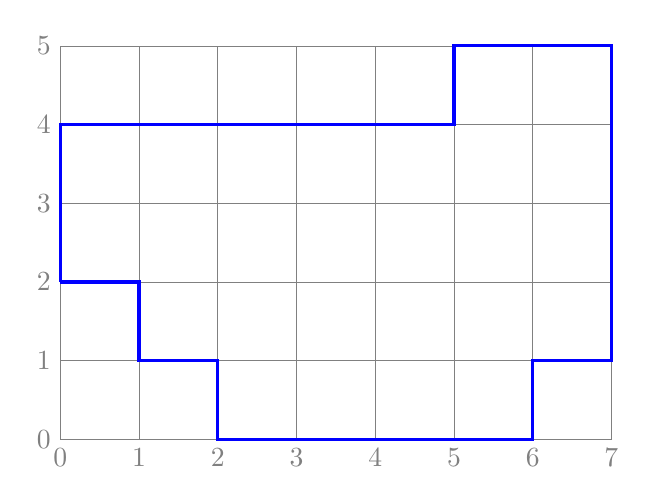
\begin{tikzpicture}[x=1cm,y=1cm]
 \newcommand*{\xMin}{0}%
\newcommand*{\xMax}{7}%
\newcommand*{\yMin}{0}%
\newcommand*{\yMax}{5}%
    \foreach \i in {\xMin,...,\xMax} {
        \draw [very thin,gray] (\i,\yMin) -- (\i,\yMax)  node [below] at (\i,\yMin) {$\i$};
    }
    \foreach \i in {\yMin,...,\yMax} {
        \draw [very thin,gray] (\xMin,\i) -- (\xMax,\i) node [left] at (\xMin,\i) {$\i$};
    }

\draw [step=1.0,blue, very thick] (0,2)-- (0,4)--(5,4)--(5,5)--(7,5)--(7,1)--(6,1)--(6,0)--(2,0)--(2,1)--(1,1)--(1,2)--(0,2) ;
\end{tikzpicture}
\end{center}
\end{example}
\begin{solution}
\begin{paracol}{2}
We could figure out the perimeter by adding up all of the edges. But there is a more clever solution. 
\switchcolumn[1]
我们可以把多边形每段边加起来。但我们还有一种比较简便的方式来求周长:把求这个多边形的周长就转化为求一个正方形的周
长,这个多边形的周长就可以巧妙地求出来了。
\end{paracol}

 \begin{center}
 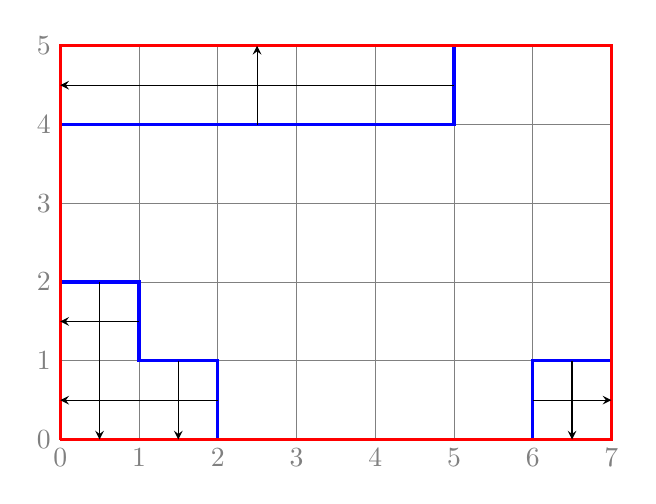
\begin{tikzpicture}[x=1cm,y=1cm]
 \newcommand*{\xMin}{0}%
\newcommand*{\xMax}{7}%
\newcommand*{\yMin}{0}%
\newcommand*{\yMax}{5}%
    \foreach \i in {\xMin,...,\xMax} {
        \draw [very thin,gray] (\i,\yMin) -- (\i,\yMax)  node [below] at (\i,\yMin) {$\i$};
    }
    \foreach \i in {\yMin,...,\yMax} {
        \draw [very thin,gray] (\xMin,\i) -- (\xMax,\i) node [left] at (\xMin,\i) {$\i$};
    }

\draw [step=1.0,blue, very thick] (0,2)-- (0,4)--(5,4)--(5,5)--(7,5)--(7,1)--(6,1)--(6,0)--(2,0)--(2,1)--(1,1)--(1,2)--(0,2) ;
\draw [step=1.0,red, very thick] (0,0) -- (0,5) -- (7,5) --(7,0) -- (0,0);
\draw [step = 1.0, black,->,>=stealth] (2.5,4)--(2.5,5);
\draw [step = 1.0, black,->,>=stealth] (5,4.5)--(0,4.5);
\draw [step = 1.0, black,->,>=stealth] (0.5,2)--(0.5,0);
\draw [step = 1.0, black,->,>=stealth] (1.5,1)--(1.5,0);
\draw [step = 1.0, black,->,>=stealth] (1,1.5)--(0,1.5);
\draw [step = 1.0, black,->,>=stealth] (2,0.5)--(0,0.5);
\draw [step = 1.0, black,->,>=stealth] (6,0.5)--(7,0.5);
\draw [step = 1.0, black,->,>=stealth] (6.5,1)--(6.5,0);
\end{tikzpicture}
\end{center}

$$
2\times(5+7) = 24.
$$
\begin{paracol}{2}
Since each of the 24 side lengths is 10 feet. The permeter is $24\times 10 = 240(feet)$. The fence cost \$ 7, so Fred's fence costs $240\times 7 = \$1680$.
\switchcolumn[1]
因为每段的长度是 10 英尺,所以周长是$24\times 10 = 240(\text{英尺})$. 每英尺围栏价格为 \$ 7, 所以 Fred 建造围栏的总花费为: $240\times 7 = \$1680$。
\end{paracol}
\end{solution}

\subsection{Area 面积}

\newpage


\chapter{Geometry 几何}


\bibliographystyle{ieeetr}
\bibliography{reference}
\addcontentsline{toc}{chapter}{参考文献}

\end{document}
